% !TEX program = xelatex
\documentclass{article}

\title{Notite examen - Algoritmi Fundamentali}
\date{}
\author{Dinu Florin-Silviu \\ grupa 231}

\newcommand{\prim}{^\ensuremath{\prime}}
\newcommand{\secund}{^{\ensuremath{\prime\prime}}}

% \makeatletter
% \renewcommand{\@seccntformat}[1]{}
% \makeatother

\newenvironment{textColor}[1]{%
    \leavevmode\color{#1}\ignorespaces%
}{%
}%


\usepackage{tikz}
\usepackage{forest}
\usepackage{hyperref}
\usepackage{amsthm}
\usepackage{amssymb}
\usepackage[english]{babel}
\usepackage[a4paper, margin=3cm]{geometry}
\usepackage{enumitem}
\usepackage{listings}
\usepackage{fontspec}
\usepackage{xcolor}
\usepackage{textcomp}
\usepackage{graphicx}
\usepackage{tabularx}

\graphicspath{ {./img/} }

\newfontfamily{\ttconsolas}{Consolas}
\lstset{
%  tabsize=4,
extendedchars=true,
        basicstyle=\ttconsolas,
        % %upquote=false,
        % aboveskip=\baselineskip,
        columns=fixed,
        showstringspaces=false,
        extendedchars=true,
        breaklines=true,
        % prebreak = \raisebox{0ex}[0ex][0ex]{\ensuremath{\hookleftarrow}},
        showtabs=false,
        showspaces=false,
        identifierstyle=\ttfamily,
        % keywordstyle=\color[rgb]{0,0,1},
        % commentstyle=\color[rgb]{0.133,0.545,0.133},
        % stringstyle=\color[rgb]{0.627,0.126,0.941},
        % language=SQL
        frame=lines,
        literate=%
    {€}{\euro}1%
    {§}{\S}1%
    {°}{\textdegree{}}1%
    {ä}{{\"a}}1%
    {ö}{{\"o}}1%
    {ü}{{\"u}}1%
    {ß}{{\ss}}1%
    {Ä}{{\"A}}1%
    {Ö}{{\"O}}1%
    {Ü}{{\"U}}1%
    {µ}{\textmu}1%
    {¹}{{\textsuperscript{1}}}1%
    {²}{{\textsuperscript{2}}}1%
    {³}{{\textsuperscript{3}}}1%
    {¼}{\textonequarter}1%
    {½}{\textonehalf}1%
    {¢}{\textcent}1%
}


\tikzstyle{red state}=[
        draw = red,
        thick,
        fill = white,
        minimum size = 4mm,
        circle
    ]

\tikzstyle{blue state}=[
    draw = blue,
    thick,
    fill = white,
    minimum size = 4mm,
    circle
]

\tikzstyle{green state}=[
    draw = green,
    thick,
    fill = white,
    minimum size = 4mm,
    circle
]

\newtheorem*{theorem}{Teorema}
\renewcommand\qedsymbol{QED}

\begin{document}
\pagenumbering{gobble}
\maketitle
\tableofcontents

\newpage
\pagenumbering{arabic}

\section{Notiuni fundamentale}
\subsection*{Grafuri izomorfe} Daca 2 grafuri:
\begin{itemize}
    \item Au acelasi numar de noduri
    \item Au acelasi numar de muchii
    \item Nodurile formeaza o secventa cu acelasi grad
    \item Daca un graf are un ciclu de lungime k, si celalalt graf are la fel
\end{itemize}

\subsection*{Grafuri bipartite} Daca un graf:
\begin{itemize}
    \item Neorientat
    \item Putem imparti nodurile in 2 multimi $V=V_1 \cup V_2$ cu $V_1 \cap V_2 = \varnothing$
    \item Fiecare muchie are o extremitate intr-o parte si cealalta in cealalta parte, adica $|e \cap V_1| = |e \cap V_2| = 1$
\end{itemize}

\subsection*{Construire graf cu secventa gradelor (Havel-Hakimi)} Ordonam descrescator gradele si incepem sa trasam muchii catre urmatoarele, scazand din gradele lor pana cand ajungem sa avem doar 0. Daca avem $d_i<0$ sau $d_i>n-1$ sau $(\sum_{i=0}^{n} d_i) \% 2 = 1$ atunci nu are solutie.

\subsection*{Levenshtein}
\begin{center}
    \[
        d_{ij} = \left\{
        \begin{array}{ll}
            j,\ i = 0                 \\
            i,\ j = 0                 \\
            d_{i-1\ j-1},\ a[i]==b[j] \\
            1 + min
            \left\{
            \begin{array}{ll}
                d_{i-1\ j} \\
                d_{i\ j-1} \\
                d_{i-1\ j-1}
            \end{array}
            \right.
        \end{array}
        \right.
    \]
\end{center}

\paragraph*{Exemplu.} Distanta dintre "examen" si "restanta"
\begin{center}
    \begin{tabularx}{0.8\textwidth} {
            | >{\centering\arraybackslash}X
            | >{\centering\arraybackslash}X
            | >{\centering\arraybackslash}X
            | >{\centering\arraybackslash}X
            | >{\centering\arraybackslash}X
            | >{\centering\arraybackslash}X
            | >{\centering\arraybackslash}X
            | >{\centering\arraybackslash}X
            |}
        \hline
          &   & e & x & a & m & e & n                           \\
        \hline
          & 0 & 1 & 2 & 3 & 4 & 5 & 6                           \\
        \hline
        r & 1 & 1 & 2 & 3 & 4 & 5 & 6                           \\
        \hline
        e & 2 & 1 & 2 & 3 & 4 & 4 & 5                           \\
        \hline
        s & 3 & 2 & 2 & 3 & 4 & 5 & 5                           \\
        \hline
        t & 4 & 3 & 3 & 3 & 4 & 5 & 6                           \\
        \hline
        a & 5 & 4 & 4 & 3 & 4 & 5 & 6                           \\
        \hline
        n & 6 & 5 & 5 & 4 & 4 & 5 & 5                           \\
        \hline
        t & 7 & 6 & 6 & 5 & 5 & 5 & 6                           \\
        \hline
        a & 8 & 7 & 7 & 6 & 6 & 6 & \textbf{\textcolor{red}{6}} \\
        \hline
    \end{tabularx}
\end{center}

\section{Parcurgeri}
\subsection*{BFS} Se iau toti vecinii nevizitati, se pun in coada, se continua cu urmatorul din coada. Complexitate $O(V+E)$. Se foloseste pentru iesirea din labirint cu drum minim si calcul nivel.
\begin{lstlisting}
void bfs(vector<vector<int>> &lista, vector<int> &pbfs, queue<int> &q) {
    int s = q.front();
    q.pop();

    int nivel = pbfs[s] + 1;

    for (auto x: lista[s]) {
        if (pbfs[x] == -1) {
            pbfs[x] = nivel;
            q.push(x);
        }
    }

    if (q.empty()) return;

    bfs(lista, pbfs, q);
}
    \end{lstlisting}

\begin{itemize}
    \item Muchiile de arbore sunt muchii din pădurea de adâncime $G_\pi$. Muchia (u, v) este o muchie de arbore dacă v a fost descoperit explorând muchia (u, v).
    \item Muchiile înapoi sunt acele muchii (u, v) care unesc un vârf u cu un strămoş v într-un arbore de adâncime. Buclele (muchii de la un vârf la el însuşi) care pot apărea într-un graf orientat sunt considerate muchii înapoi.
    \item Muchiile înainte sunt acele muchii (u, v) ce nu sunt muchii de arbore şi conectează un vârf u cu un descendent v într-un arbore de adâncime.
    \item Muchiile transversale sunt toate celelalte muchii. Ele pot uni vârfuri din acelaşi arbore de adâncime, cu condiţia ca unul să nu fie strămoşul celuilalt, sau pot uni vârfuri din arbori, de adâncime, diferiţi.
\end{itemize}

\subsection*{DFS} Complexitate $O(V+E)$.
\begin{lstlisting}
void Graph::DFS(int v)
{
    // Mark the current node as visited and
    // print it
    visited[v] = true;
    cout << v << " ";
 
    // Recur for all the vertices adjacent
    // to this vertex
    list<int>::iterator i;
    for (i = adj[v].begin(); i != adj[v].end(); ++i)
        if (!visited[*i])
            DFS(*i);
}
    \end{lstlisting}

\section{Sortare topologica}
Se face pe DAG (directed acyclic graph)
\subsection*{Cu BFS} Incepe de la toate nodurile care au $indegree == 0$ (DAG garanteaza cel putin 1 astfel de nod). Dupa ce scoatem nodul din coada, il punem in vector. Pentru fiecare vecin, scad indegree curent. Daca dupa scadere, vecinul are indegree 0, il adaug in coada.
\begin{lstlisting}
vector<int> topo(int N, vector<int> adj[]) {
    queue<int> q; 
    vector<int> indegree(N, 0); 
    for(int i = 0;i<N;i++) {
        for(auto it: adj[i]) {
            indegree[it]++; 
        }
    }
    
    for(int i = 0;i<N;i++) {
        if(indegree[i] == 0) {
            q.push(i); 
        }
    }
    vector<int> topo;
    while(!q.empty()) {
        int node = q.front(); 
        q.pop(); 
        topo.push_back(node);
        for(auto it : adj[node]) {
            indegree[it]--;
            if(indegree[it] == 0) {
                q.push(it); 
            }
        }
    }
    return topo;
}
    \end{lstlisting}
\subsection*{Cu DFS} Diferentea fata de DFS e ca pun la sfarsit nodul pe stack. Diferentele fata de anterior sunt ca iau tot ce nu e vizitat si ca e mai eficient dpdv al memoriei, cat timp lantul cel mai lung nu da stackoverflow. Complexitate $O(V+E)$

\begin{lstlisting}
void Graph::topologicalSortUtil(int v, bool visited[],
                                stack<int>& Stack)
{
    // Mark the current node as visited.
    visited[v] = true;
 
    // Recur for all the vertices
    // adjacent to this vertex
    list<int>::iterator i;
    for (i = adj[v].begin(); i != adj[v].end(); ++i)
        if (!visited[*i])
            topologicalSortUtil(*i, visited, Stack);
 
    // Push current vertex to stack
    // which stores result
    Stack.push(v);
}
    \end{lstlisting}

\section{Muchii critice} Acele muchii care nu fac parte dintr-un ciclu. Facem un DFS si tinem 2 valori: low si disc. Pentru fiecare nod, mai intai punem disc ca fiind $disc_{anterior} + 1$, trecem la copil, pentru el memoram parintele, apoi facem DFS, apoi actualizam low ca fiind $min(low[copil], low[parinte])$. Daca este critica, atunci $low[copil]>disc[parinte]$.
\paragraph*{Algoritm.}
\begin{itemize}
    \item Marcam nodul ca vizitat
    \item disc = low = ++time
    \item Iteram prin vecini
    \item Daca vecinul e nevizitat
          \begin{itemize}
              \item Facem DFS cu primul pas
              \item low va fi minimul dintre low-ul curent si cel al vecinului vizitat recent
              \item daca low-ul vecin < disc curent, e muchie critica intre ele
          \end{itemize}
    \item Daca vecinul este vizitat si nu e parinte, atunci low va fi minimul dintre low-ul curent si disc-ul vecinului
\end{itemize}
\begin{lstlisting}
void Graph::bridgeUtil(int u, bool visited[], int disc[],
                                  int low[], int parent[])
{
    // A static variable is used for simplicity, we can
    // avoid use of static variable by passing a pointer.
    static int time = 0;
 
    // Mark the current node as visited
    visited[u] = true;
 
    // Initialize discovery time and low value
    disc[u] = low[u] = ++time;
 
    // Go through all vertices adjacent to this
    list<int>::iterator i;
    for (i = adj[u].begin(); i != adj[u].end(); ++i)
    {
        int v = *i;  // v is current adjacent of u
 
        // If v is not visited yet, then recur for it
        if (!visited[v])
        {
            parent[v] = u;
            bridgeUtil(v, visited, disc, low, parent);
 
            // Check if the subtree rooted with v has a
            // connection to one of the ancestors of u
            low[u]  = min(low[u], low[v]);
 
            // If the lowest vertex reachable from subtree
            // under v is  below u in DFS tree, then u-v
            // is a bridge
            if (low[v] > disc[u])
              cout << u <<" " << v << endl;
        }
 
        // Update low value of u for parent function calls.
        else if (v != parent[u])
            low[u]  = min(low[u], disc[v]);
    }
}
    \end{lstlisting}

\section{Puncte critice} V este punct critic, daca exista 2 noduri x si y, cu $x,y \neq v$, pentru care v apartine oricarui $x,y-lant$

\paragraph*{Teorema.} $\forall$ graf conectat non-trivial contine $\geq 2$ noduri care NU sunt puncte critice.

\paragraph*{Algoritm.}
\begin{itemize}
    \item Memoram nodul ca fiind vizitat
    \item disc = low = ++time
    \item Iteram prin vecini
    \item Daca vecinul e nevizitat
          \begin{itemize}
              \item Incrementam nr de copii
              \item DFS cu primul pas pe nodul nevizitat cu parintele incrementat cu 1
              \item low curent va fi minimul dintre low curent si low copil
              \item Daca \textbf{NU E RADACINA} si disc-ul curent $\leq$ low-ul copilului, atunci e punct critic
          \end{itemize}
    \item Daca e nevizitat, atunci low-ul curent va fi minimul dintre low-ul curent si disc-ul copilului
    \item Daca dupa parcurgerea vecinilor, vedem ca e radacina si are $\geq 2$ copii vizitati direct, atunci e punct de articulatie
\end{itemize}

\begin{lstlisting}
void APUtil(vector<int> adj[], int u, bool visited[],
    int disc[], int low[], int& time, int parent,
    bool isAP[])
{
// Count of children in DFS Tree
int children = 0;

// Mark the current node as visited
visited[u] = true;

// Initialize discovery time and low value
disc[u] = low[u] = ++time;

// Go through all vertices adjacent to this
for (auto v : adj[u]) {
// If v is not visited yet, then make it a child of u
// in DFS tree and recur for it
if (!visited[v]) {
    children++;
    APUtil(adj, v, visited, disc, low, time, u, isAP);

    // Check if the subtree rooted with v has
    // a connection to one of the ancestors of u
    low[u] = min(low[u], low[v]);

    // If u is not root and low value of one of
    // its child is more than discovery value of u.
    if (parent != -1 && low[v] >= disc[u])
        isAP[u] = true;
}

// Update low value of u for parent function calls.
else if (v != parent)
    low[u] = min(low[u], disc[v]);
}

// If u is root of DFS tree and has two or more children.
if (parent == -1 && children > 1)
isAP[u] = true;
}

void AP(vector<int> adj[], int V)
{
int disc[V] = { 0 };
int low[V];
bool visited[V] = { false };
bool isAP[V] = { false };
int time = 0, par = -1;

// Adding this loop so that the
// code works even if we are given
// disconnected graph
for (int u = 0; u < V; u++)
if (!visited[u])
    APUtil(adj, u, visited, disc, low,
           time, par, isAP);

// Printing the APs
for (int u = 0; u < V; u++)
if (isAP[u] == true)
    cout << u << " ";
}
    \end{lstlisting}

\section{Conexitate in graf orientat} Exista 2 tipuri de conexitati intr-un graf orientat:
\begin{itemize}
    \item Slab conex: Drum de intre $\forall$ 2 noduri daca consideram graful neorientat
    \item Tare conex: Drum intre $\forall$ 2 noduri
\end{itemize}

\subsection*{Kosaraju} Fac un DFS in care adaug pe stack nodurile. Transpun graful. Popuiesc stackul, fac DFS pe acel nod in care marchez elementele ca vizitate, apoi popuiesc urmatorul element si fac DFS daca e nevizitat. Complexitate $O(V+E)$.

\begin{lstlisting}
#include <bits/stdc++.h>

#define MAX_N 20001
#define ll long long int
using namespace std;
int n, m;

struct Node {
  vector < int > adj;
  vector < int > rev_adj;
};

Node g[MAX_N];

stack < int > S;
bool visited[MAX_N];

int component[MAX_N];
vector < int > components[MAX_N];
int numComponents;

void dfs_1(int x) {
  visited[x] = true;
  for (int i = 0; i < g[x].adj.size(); i++) {
    if (!visited[g[x].adj[i]]) dfs_1(g[x].adj[i]);
  }
  S.push(x);
}

void dfs_2(int x) {
  printf("%d ", x);
  component[x] = numComponents;
  components[numComponents].push_back(x);
  visited[x] = true;
  for (int i = 0; i < g[x].rev_adj.size(); i++) {
    if (!visited[g[x].rev_adj[i]]) dfs_2(g[x].rev_adj[i]);
  }
}

void Kosaraju() {
  for (int i = 0; i < n; i++)
    if (!visited[i]) dfs_1(i);

  for (int i = 0; i < n; i++)
    visited[i] = false;

  while (!S.empty()) {
    int v = S.top();
    S.pop();
    if (!visited[v]) {
      printf("Component %d: ", numComponents);
      dfs_2(v);
      numComponents++;
      printf("\n");
    }
  }
}

int main() {

  cin >> n >> m;
  int a, b;
  while (m--) {
    cin >> a >> b;
    g[a].adj.push_back(b);
    g[b].rev_adj.push_back(a);
  }

  Kosaraju();
  printf("Total number of components: %d\n", numComponents);

  return 0;
}

\end{lstlisting}

\paragraph*{Algoritmul lui Tarjan.} Complexitate $O(V+E)$
\begin{lstlisting}
void Graph::SCCUtil(int u, int disc[], int low[],
        stack<int>* st, bool stackMember[])
    {
        // A static variable is used for simplicity, we can
        // avoid use of static variable by passing a pointer.
        static int time = 0;
    
        // Initialize discovery time and low value
        disc[u] = low[u] = ++time;
        st->push(u);
        stackMember[u] = true;
    
        // Go through all vertices adjacent to this
        list<int>::iterator i;
        for (i = adj[u].begin(); i != adj[u].end(); ++i) {
            int v = *i; // v is current adjacent of 'u'
    
            // If v is not visited yet, then recur for it
            if (disc[v] == -1) {
                SCCUtil(v, disc, low, st, stackMember);
    
                // Check if the subtree rooted with 'v' has a
                // connection to one of the ancestors of 'u'
                // Case 1 (per above discussion on Disc and Low
                // value)
                low[u] = min(low[u], low[v]);
            }
    
            // Update low value of 'u' only of 'v' is still in
            // stack (i.e. it's a back edge, not cross edge).
            // Case 2 (per above discussion on Disc and Low
            // value)
            else if (stackMember[v] == true)
            low[u] = min(low[u], disc[v]);
        }
    
        // head node found, pop the stack and print an SCC
        int w = 0; // To store stack extracted vertices
        if (low[u] == disc[u]) {
            while (st->top() != u) {
                w = (int)st->top();
                cout << w << " ";
                stackMember[w] = false;
                st->pop();
            }
            w = (int)st->top();
            cout << w << "\n";
            stackMember[w] = false;
            st->pop();
        }
    }
    
    // The function to do DFS traversal. It uses SCCUtil()
    void Graph::SCC()
    {
        int* disc = new int[V];
        int* low = new int[V];
        bool* stackMember = new bool[V];
        stack<int>* st = new stack<int>();
    
        // Initialize disc and low, and stackMember arrays
        for (int i = 0; i < V; i++) {
            disc[i] = NIL;
            low[i] = NIL;
            stackMember[i] = false;
        }
    
        // Call the recursive helper function to find strongly
        // connected components in DFS tree with vertex 'i'
        for (int i = 0; i < V; i++)
            if (disc[i] == NIL)
                SCCUtil(i, disc, low, st, stackMember);
    }
\end{lstlisting}

\subsection*{Lema} Dacă două vârfuri se află în aceeaşi componentă tare conexă, atunci
nici un drum între ele nu părăseşte, vreodată, componentă tare conexă.
\\
\textbf{Demonstrație:} Fie u și v două noduri din componenta tare conexă.
Presupunem ca exista w în afara componentei și există drum u - > v prin w.
Atunci avem drum de la u la w dar avem și drumul w->v->u deci și drum de la
w la u deci w este în componenta tare conexă.

\section{APM - arbori partiali de cost minim}
\subsection*{Kruskal} $O(E*log E+ E*log V)$ Algoritmul are 3 pasi:
\begin{itemize}
    \item Sorteaza toate muchiile in oridinea crescatoare a greutatii
    \item Alege muchia cea mai mica, daca formeaza un ciclu, treci la urmatoarea, daca nu, adaug-o.
    \item Repeta pasul anterior pana ai $V - 1$ muchii.
\end{itemize}

\paragraph*{Exemplu} Fie graful

\begin{center}
    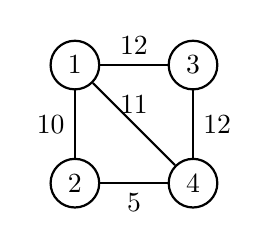
\begin{tikzpicture}[node distance={15mm}, thick, main/.style = {draw, circle}]
        \node[main] (1) {1};
        \node[main] (2) [below of = 1] {2};
        \node[main] (3) [right of = 1] {3};
        \node[main] (4) [below of = 3]{4};

        \draw[-] (1) -- (2) node [midway,left] {10};
        \draw[-] (2) -- (4) node [midway, below] {5};
        \draw[-] (3) -- (4) node [midway, right] {12};
        \draw[-] (1) -- (4) node [midway, right, above] {11};
        \draw[-] (1) -- (3) node [midway, above] {12};

    \end{tikzpicture}
\end{center}

\subparagraph*{Pasul 1.} Sortam ASC muchiile: $\{(2,4,5), (1,2,10), (1,4,11), (1,3,12), (3,4,12)\}$. Am folosit notatia $(nod1, nod2, greutate)$.
\subparagraph*{Pasii 2 \& 3.}
\subparagraph*{1.} Incepem recursia alegand cea mai mica muchie $(2,4,5)$.

\begin{center}
    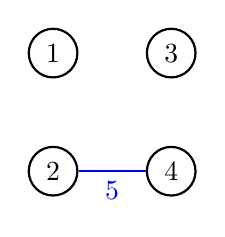
\begin{tikzpicture}[node distance={15mm}, thick, main/.style = {draw, circle}]
        \node[main] (1) {1};
        \node[main] (2) [below of = 1] {2};
        \node[main] (3) [right of = 1] {3};
        \node[main] (4) [below of = 3]{4};

        \draw[blue] (2) -- (4) node [midway, below] {5};

    \end{tikzpicture}
\end{center}

\subparagraph*{2.} Continuam cu $(1,2,10)$.

\begin{center}
    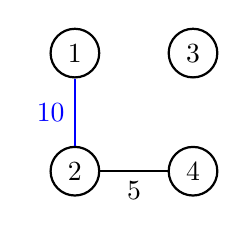
\begin{tikzpicture}[node distance={15mm}, thick, main/.style = {draw, circle}]
        \node[main] (1) {1};
        \node[main] (2) [below of = 1] {2};
        \node[main] (3) [right of = 1] {3};
        \node[main] (4) [below of = 3]{4};

        \draw[-] (2) -- (4) node [midway, below] {5};
        \draw[blue] (1) -- (2) node [midway,left] {10};

    \end{tikzpicture}
\end{center}

\subparagraph*{3.} Continuam cu $(1,4,11)$.

\begin{center}
    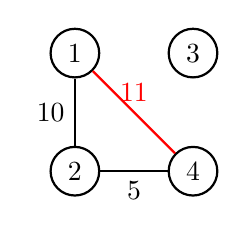
\begin{tikzpicture}[node distance={15mm}, thick, main/.style = {draw, circle}]
        \node[main] (1) {1};
        \node[main] (2) [below of = 1] {2};
        \node[main] (3) [right of = 1] {3};
        \node[main] (4) [below of = 3]{4};

        \draw[-] (2) -- (4) node [midway, below] {5};
        \draw[-] (1) -- (2) node [midway,left] {10};
        \draw[red] (1) -- (4) node [midway, right, above] {11};

    \end{tikzpicture}
\end{center}

\begin{center}
    \textbf{Observam ca face ciclu, deci o ignoram}
\end{center}

\begin{center}
    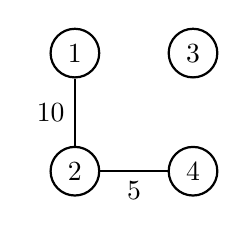
\begin{tikzpicture}[node distance={15mm}, thick, main/.style = {draw, circle}]
        \node[main] (1) {1};
        \node[main] (2) [below of = 1] {2};
        \node[main] (3) [right of = 1] {3};
        \node[main] (4) [below of = 3]{4};

        \draw[-] (2) -- (4) node [midway, below] {5};
        \draw[-] (1) -- (2) node [midway,left] {10};

    \end{tikzpicture}
\end{center}

\subparagraph*{4.} Continuam cu $(1,3,12)$.

\begin{center}
    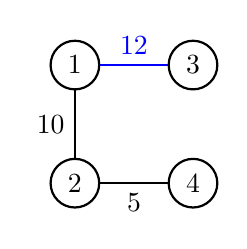
\begin{tikzpicture}[node distance={15mm}, thick, main/.style = {draw, circle}]
        \node[main] (1) {1};
        \node[main] (2) [below of = 1] {2};
        \node[main] (3) [right of = 1] {3};
        \node[main] (4) [below of = 3]{4};

        \draw[-] (2) -- (4) node [midway, below] {5};
        \draw[-] (1) -- (2) node [midway,left] {10};
        \draw[blue] (1) -- (3) node [midway, above] {12};

    \end{tikzpicture}
\end{center}

\begin{center}
    \textbf{Observam ca avem $V-1$ muchii, deci ramanem cu acest graf}
\end{center}

\subparagraph*{K-clustering (aplicatie)} Imparte in k clustere (are $n-k$ pasi)
\begin{center}
    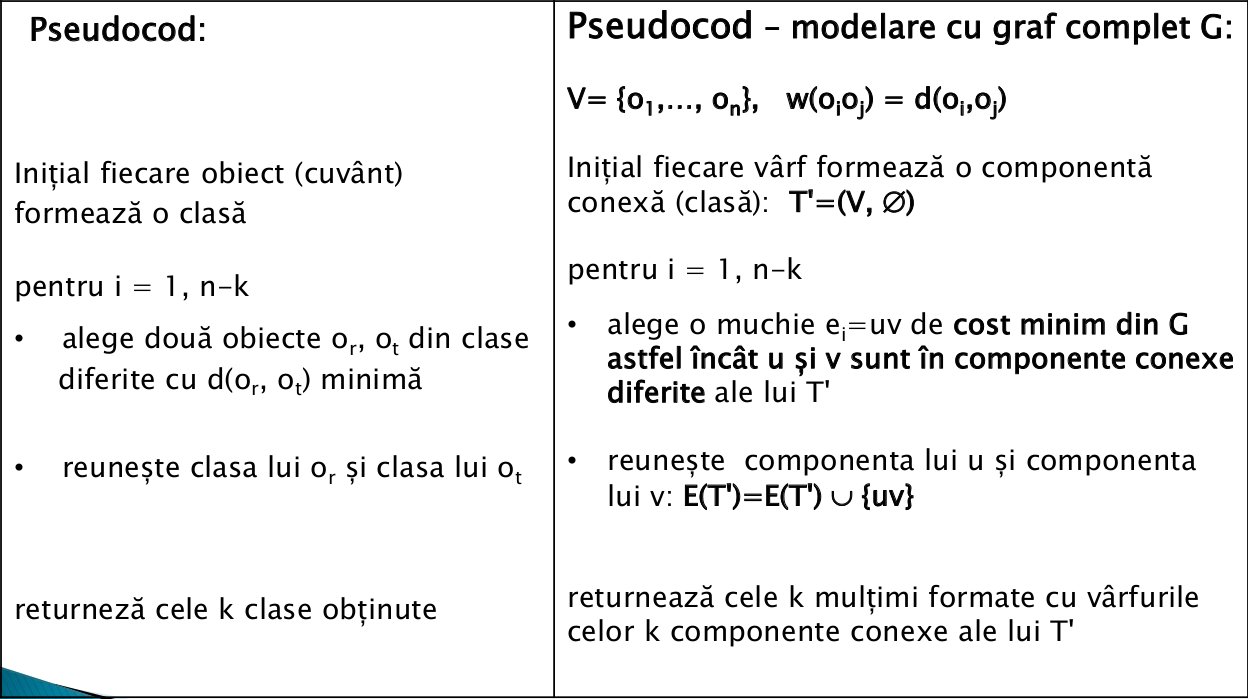
\includegraphics[scale=0.3]{1_kclustering.png}
\end{center}

\subsection*{Prim} Complexitate $O(V^2)$ sau $O(V*logV + E*logV)$ daca folosim minheap. Algoritmul are 6 pasi:
\begin{itemize}
    \item Alegem un nod $n$ aleatoriu si il scoatem din lista nodurilor de ales
    \item Adaugam in structura de date toti vecinii sai impreuna cu greutatea muchiilor
    \item Actualizam eticheta pentru fiecare varf cu distanta minima fata de cele incluse in graf
    \item Adaugam nodul cu distanta minima cea mai mica, il scaotem din lista nodurilor de ales si ii facem parintele nodul de care se leaga
    \item Adaugam in structura de date toti vecinii sai impreuna cu greutatea muchiilor
    \item Repetam al 4-lea pas.
\end{itemize}

\begin{center}
    \includegraphics*[scale=0.3]{2_prim.png}
\end{center}
\begin{center}
    \textbf{$\uparrow$ Prim prin vector vizitat $\uparrow$}
\end{center}


\paragraph*{Exemplu} Fie graful

\begin{center}
    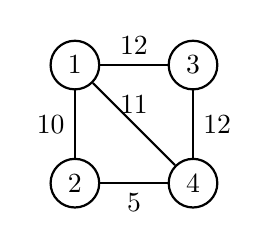
\begin{tikzpicture}[node distance={15mm}, thick, main/.style = {draw, circle}]
        \node[main] (1) {1};
        \node[main] (2) [below of = 1] {2};
        \node[main] (3) [right of = 1] {3};
        \node[main] (4) [below of = 3]{4};

        \draw[-] (1) -- (2) node [midway,left] {10};
        \draw[-] (2) -- (4) node [midway, below] {5};
        \draw[-] (3) -- (4) node [midway, right] {12};
        \draw[-] (1) -- (4) node [midway, right, above] {11};
        \draw[-] (1) -- (3) node [midway, above] {12};

    \end{tikzpicture}
\end{center}

\subparagraph*{Pasul 1.} Plecam de la nodul 1 si facem urmatoarea structura

\begin{center}
    $[(d/tata)] = \{(0,0),(\infty,0),(\infty,0),(\infty,0)\}$
\end{center}

\subparagraph*{Pasul 2.}
\begin{center}
    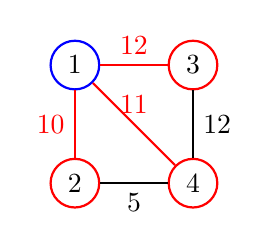
\begin{tikzpicture}[node distance={15mm}, thick, main/.style = {draw, circle}]
        \node[blue state] (1) {1};
        \node[red state] (2) [below of = 1] {2};
        \node[red state] (3) [right of = 1] {3};
        \node[red state] (4) [below of = 3]{4};

        \draw[red] (1) -- (2) node [midway,left] {10};
        \draw[-] (2) -- (4) node [midway, below] {5};
        \draw[-] (3) -- (4) node [midway, right] {12};
        \draw[red] (1) -- (4) node [midway, right, above] {11};
        \draw[red] (1) -- (3) node [midway, above] {12};

    \end{tikzpicture}
\end{center}

\subparagraph*{Pasul 3.}
\begin{center}
    $[(d/tata)] = \{(0,0),(10,0),(12,0),(11,0)\}$
\end{center}

\subparagraph*{Pasul 4.}
\begin{center}
    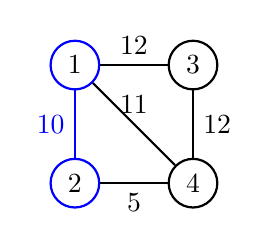
\begin{tikzpicture}[node distance={15mm}, thick, main/.style = {draw, circle}]
        \node[blue state] (1) {1};
        \node[blue state] (2) [below of = 1] {2};
        \node[main] (3) [right of = 1] {3};
        \node[main] (4) [below of = 3]{4};

        \draw[blue] (1) -- (2) node [midway,left] {10};
        \draw[-] (2) -- (4) node [midway, below] {5};
        \draw[-] (3) -- (4) node [midway, right] {12};
        \draw[-] (1) -- (4) node [midway, right, above] {11};
        \draw[-] (1) -- (3) node [midway, above] {12};

    \end{tikzpicture}
\end{center}

\subparagraph*{Pasul 5.}

\begin{center}
    $[(d/tata)] = \{(0,0),(10,1),(12,0),(5,0)\}$
\end{center}

\subparagraph*{Pasul 6. Repetam}

\begin{center}
    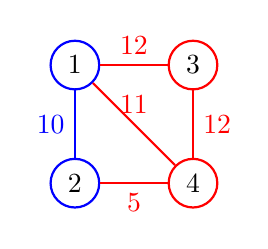
\begin{tikzpicture}[node distance={15mm}, thick, main/.style = {draw, circle}]
        \node[blue state] (1) {1};
        \node[blue state] (2) [below of = 1] {2};
        \node[red state] (3) [right of = 1] {3};
        \node[red state] (4) [below of = 3]{4};

        \draw[blue] (1) -- (2) node [midway,left] {10};
        \draw[red] (2) -- (4) node [midway, below] {5};
        \draw[red] (3) -- (4) node [midway, right] {12};
        \draw[red] (1) -- (4) node [midway, right, above] {11};
        \draw[red] (1) -- (3) node [midway, above] {12};

    \end{tikzpicture}
\end{center}

\begin{center}
    $[(d/tata)] = \{(0,0),(10,1),(12,0),(5,0)\}$
\end{center}

\begin{center}
    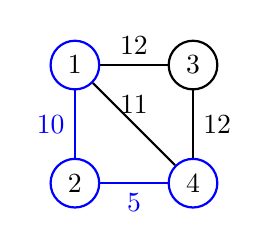
\begin{tikzpicture}[node distance={15mm}, thick, main/.style = {draw, circle}]
        \node[blue state] (1) {1};
        \node[blue state] (2) [below of = 1] {2};
        \node[main] (3) [right of = 1] {3};
        \node[blue state] (4) [below of = 3]{4};

        \draw[blue] (1) -- (2) node [midway,left] {10};
        \draw[blue] (2) -- (4) node [midway, below] {5};
        \draw[-] (3) -- (4) node [midway, right] {12};
        \draw[-] (1) -- (4) node [midway, right, above] {11};
        \draw[-] (1) -- (3) node [midway, above] {12};

    \end{tikzpicture}
\end{center}

\begin{center}
    $[(d/tata)] = \{(0,0),(10,1),(12,0),(5,2)\}$
\end{center}

\begin{center}
    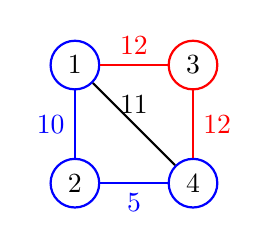
\begin{tikzpicture}[node distance={15mm}, thick, main/.style = {draw, circle}]
        \node[blue state] (1) {1};
        \node[blue state] (2) [below of = 1] {2};
        \node[red state] (3) [right of = 1] {3};
        \node[blue state] (4) [below of = 3]{4};

        \draw[blue] (1) -- (2) node [midway,left] {10};
        \draw[blue] (2) -- (4) node [midway, below] {5};
        \draw[red] (3) -- (4) node [midway, right] {12};
        \draw[-] (1) -- (4) node [midway, right, above] {11};
        \draw[red] (1) -- (3) node [midway, above] {12};

    \end{tikzpicture}
\end{center}

\begin{center}
    $[(d/tata)] = \{(0,0),(10,1),(12,0),(5,2)\}$
\end{center}

\begin{center}
    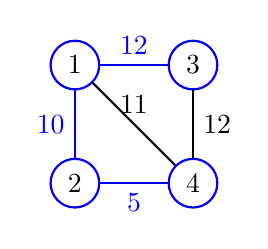
\begin{tikzpicture}[node distance={15mm}, thick, main/.style = {draw, circle}]
        \node[blue state] (1) {1};
        \node[blue state] (2) [below of = 1] {2};
        \node[blue state] (3) [right of = 1] {3};
        \node[blue state] (4) [below of = 3]{4};

        \draw[blue] (1) -- (2) node [midway,left] {10};
        \draw[blue] (2) -- (4) node [midway, below] {5};
        \draw[-] (3) -- (4) node [midway, right] {12};
        \draw[-] (1) -- (4) node [midway, right, above] {11};
        \draw[blue] (1) -- (3) node [midway, above] {12};

    \end{tikzpicture}
\end{center}

\begin{center}
    $[(d/tata)] = \{(0,0),(10,1),(12,1),(5,2)\}$
\end{center}

\begin{center}
    \textbf{APM final}
\end{center}

\begin{center}
    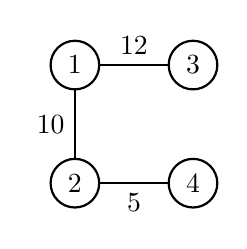
\begin{tikzpicture}[node distance={15mm}, thick, main/.style = {draw, circle}]
        \node[main] (1) {1};
        \node[main] (2) [below of = 1] {2};
        \node[main] (3) [right of = 1] {3};
        \node[main] (4) [below of = 3]{4};

        \draw[-] (1) -- (2) node [midway,left] {10};
        \draw[-] (2) -- (4) node [midway, below] {5};
        \draw[-] (1) -- (3) node [midway, above] {12};

    \end{tikzpicture}
\end{center}

\begin{center}
    \includegraphics*[scale=0.3]{3_prim_minheap.png}
\end{center}
\begin{center}
    \textbf{$\uparrow$ Prim prin minheap $\uparrow$}
\end{center}

\section{Drumuri minime de sursa unica \textit{s}}
\subsection*{Dijkstra}
Se poate folosi doar pentru drumuri de cost pozitiv
\paragraph*{Complexitate}
\begin{itemize}
    \item Cu heap $O(E*logV)$
          \begin{itemize}
              \item Initializare Q: $O(n)$
              \item n * extragere varf minim: $O(n*log\ n)$
              \item Actualizare etichete vecini: $O(n*log\ n)$
          \end{itemize}
    \item Cu vector $O(V^2)$
          \begin{itemize}
              \item Initializare Q: $O(n)$
              \item n * extragere varf minim: $O(n^2)$
              \item Actualizare etichete vecini: $O(m^2)$
          \end{itemize}
\end{itemize}
\begin{center}
    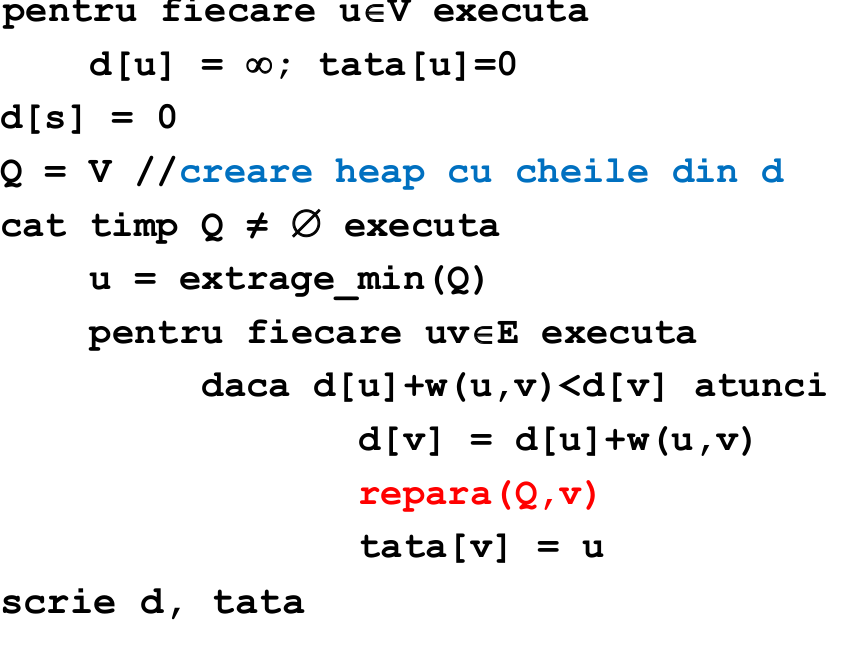
\includegraphics[scale=0.3]{4_dijkstra.png}
\end{center}
\begin{center}
    \textbf{$\uparrow$ Dijskstra cu min heap $\uparrow$}
\end{center}

\begin{center}
    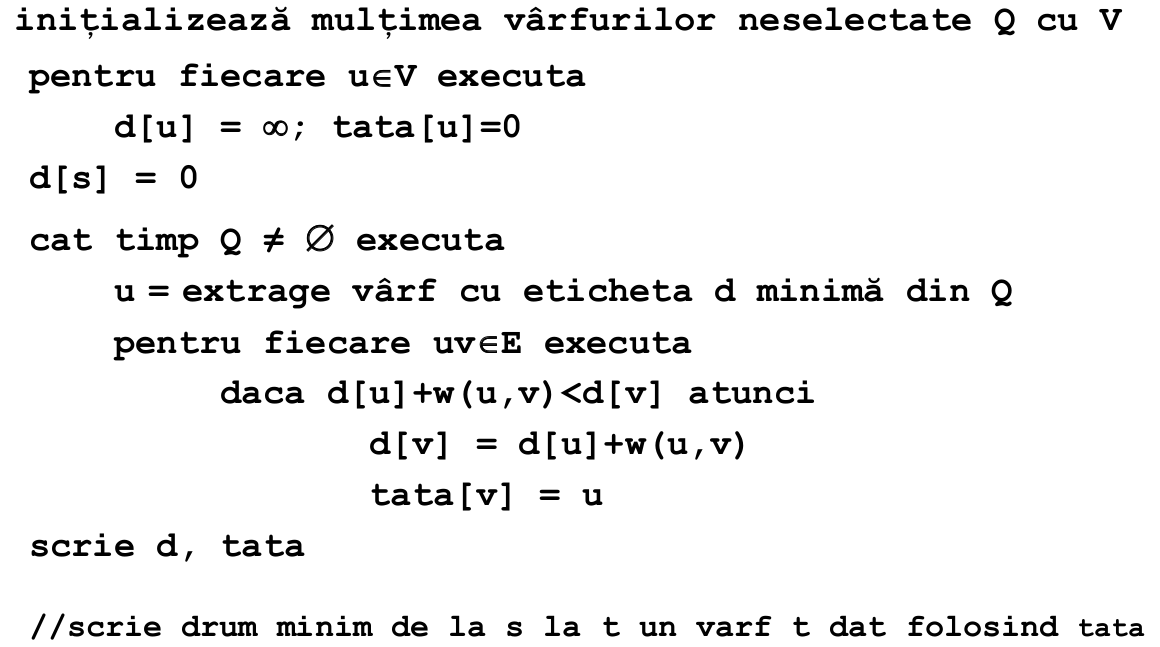
\includegraphics[scale=0.3]{5_dijkstra_vector.png}
\end{center}
\begin{center}
    \textbf{$\uparrow$ Dijskstra cu vector $\uparrow$}
\end{center}

\paragraph*{Exemplu} Fie graful in care incepem de la 1.

\begin{center}
    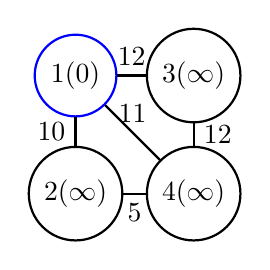
\begin{tikzpicture}[node distance={15mm}, thick, main/.style = {draw, circle}]
        \node[blue state] (1) {1(0)};
        \node[main] (2) [below of = 1] {2($\infty$)};
        \node[main] (3) [right of = 1] {3($\infty$)};
        \node[main] (4) [below of = 3]{4($\infty$)};

        \draw[-] (1) -- (2) node [midway,left] {10};
        \draw[-] (2) -- (4) node [midway, below] {5};
        \draw[-] (3) -- (4) node [midway, right] {12};
        \draw[-] (1) -- (4) node [midway, right, above] {11};
        \draw[-] (1) -- (3) node [midway, above] {12};

    \end{tikzpicture}
\end{center}

\subparagraph*{Consideram vecinii lui 1}
\begin{center}
    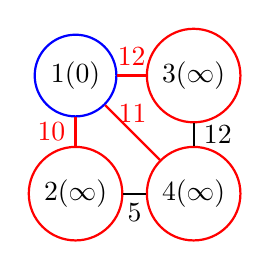
\begin{tikzpicture}[node distance={15mm}, thick, main/.style = {draw, circle}]
        \node[blue state] (1) {1(0)};
        \node[red state] (2) [below of = 1] {2($\infty$)};
        \node[red state] (3) [right of = 1] {3($\infty$)};
        \node[red state] (4) [below of = 3]{4($\infty$)};

        \draw[red] (1) -- (2) node [midway,left] {10};
        \draw[-] (2) -- (4) node [midway, below] {5};
        \draw[-] (3) -- (4) node [midway, right] {12};
        \draw[red] (1) -- (4) node [midway, right, above] {11};
        \draw[red] (1) -- (3) node [midway, above] {12};

    \end{tikzpicture}
\end{center}

\subparagraph*{Actualizam distantele vecinilor lui 1 si il alegem pe minimul nevizitat (2)}
\begin{center}
    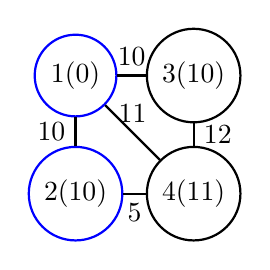
\begin{tikzpicture}[node distance={15mm}, thick, main/.style = {draw, circle}]
        \node[blue state] (1) {1(0)};
        \node[blue state] (2) [below of = 1] {2(10)};
        \node[main] (3) [right of = 1] {3(10)};
        \node[main] (4) [below of = 3]{4(11)};

        \draw[-] (1) -- (2) node [midway,left] {10};
        \draw[-] (2) -- (4) node [midway, below] {5};
        \draw[-] (3) -- (4) node [midway, right] {12};
        \draw[-] (1) -- (4) node [midway, right, above] {11};
        \draw[-] (1) -- (3) node [midway, above] {10};

    \end{tikzpicture}
\end{center}

\subparagraph*{Actualizam distantele vecinilor lui 2 si il luam pe minimul nevizitat (3)}

\begin{center}
    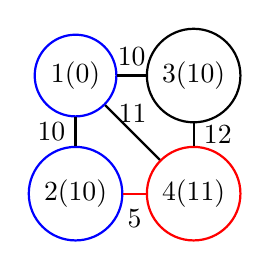
\begin{tikzpicture}[node distance={15mm}, thick, main/.style = {draw, circle}]
        \node[blue state] (1) {1(0)};
        \node[blue state] (2) [below of = 1] {2(10)};
        \node[main] (3) [right of = 1] {3(10)};
        \node[red state] (4) [below of = 3]{4(11)};

        \draw[-] (1) -- (2) node [midway,left] {10};
        \draw[red state] (2) -- (4) node [midway, below] {5};
        \draw[-] (3) -- (4) node [midway, right] {12};
        \draw[-] (1) -- (4) node [midway, right, above] {11};
        \draw[-] (1) -- (3) node [midway, above] {10};

    \end{tikzpicture}
\end{center}

\subparagraph*{Actualizam distantele vecinilor lui 2 si il luam pe minimul nevizitat (4)}

\begin{center}
    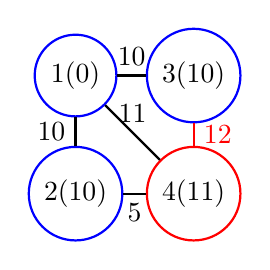
\begin{tikzpicture}[node distance={15mm}, thick, main/.style = {draw, circle}]
        \node[blue state] (1) {1(0)};
        \node[blue state] (2) [below of = 1] {2(10)};
        \node[blue state] (3) [right of = 1] {3(10)};
        \node[red state] (4) [below of = 3]{4(11)};

        \draw[-] (1) -- (2) node [midway,left] {10};
        \draw[-] (2) -- (4) node [midway, below] {5};
        \draw[red] (3) -- (4) node [midway, right] {12};
        \draw[-] (1) -- (4) node [midway, right, above] {11};
        \draw[-] (1) -- (3) node [midway, above] {10};

    \end{tikzpicture}
\end{center}

\subparagraph*{Luam minimul nevizitat si vedem ca nu mai are vecini}

\begin{center}
    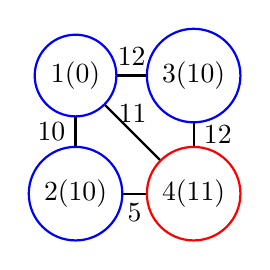
\begin{tikzpicture}[node distance={15mm}, thick, main/.style = {draw, circle}]
        \node[blue state] (1) {1(0)};
        \node[blue state] (2) [below of = 1] {2(10)};
        \node[blue state] (3) [right of = 1] {3(10)};
        \node[red state] (4) [below of = 3]{4(11)};

        \draw[-] (1) -- (2) node [midway,left] {10};
        \draw[-] (2) -- (4) node [midway, below] {5};
        \draw[-] (3) -- (4) node [midway, right] {12};
        \draw[-] (1) -- (4) node [midway, right, above] {11};
        \draw[-] (1) -- (3) node [midway, above] {12};

    \end{tikzpicture}
\end{center}

\paragraph*{Lema}
Pentru $\forall u\in V$, la orice pas al algoritmului lui Dijkstra avem:
\begin{itemize}
    \item dacă $d[u]<\infty$, există un drum de la s la u în G de cost d[u] și acesta se poate determina din vectorul tata: \\ tata[u]= predecesorul lui u pe un drum de la s la u de cost d[u]
    \item $d[u] \leq \delta(s,u)$
\end{itemize}
\subparagraph*{Consecinta} Dacă la un pas al algoritmului avem pentru un vârf u relația $d[u] = \delta(s, u)$, atunci d[u] nu se mai modifică până la final.

\paragraph*{Teorema} Fie G=(V, E, w) un graf orientat ponderat cu $w : E \to \mathbb{R}_+$ și $s \in V$ fixat.\\
La finalul algoritmul lui Dijkstra avem:
$d[u] = \delta(s, u)$ pentru orice $u \in V$ și tata memorează un arbore al distanțelor față de s.

\subsection*{Bellman-Ford}
Se poate folosi si pentru drumuri negative
\paragraph*{Complexitate} $O(V*E)$
\begin{center}
    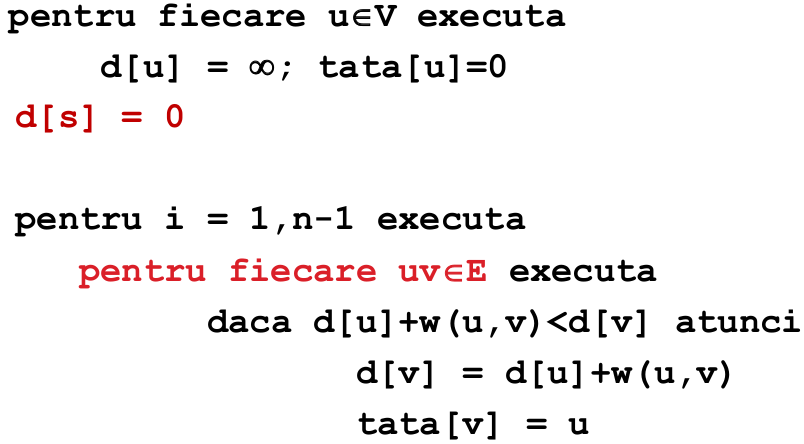
\includegraphics[scale=0.3]{6_bellmanford.png}
\end{center}

\paragraph*{Optimizare} Se pot relaxa doar arcele din varfurile ale caror etichete s-au modificat anterior

\paragraph*{Exemplu}
\begin{center}
    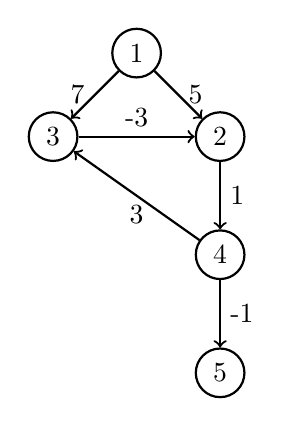
\begin{tikzpicture}[node distance={15mm}, thick, main/.style = {draw, circle}]
        \node[main] (1) {1};
        \node[main] (2) [below right of = 1] {2};
        \node[main] (3) [below left of = 1] {3};
        \node[main] (4) [below of = 2]{4};
        \node[main] (5) [below of = 4]{5};

        \draw[->] (1) -- (2) node [midway,right] {5};
        \draw[->] (1) -- (3) node [midway, left] {7};
        \draw[->] (2) -- (4) node [midway, right] {1};
        \draw[->] (4) -- (5) node [midway, right] {-1};
        \draw[->] (3) -- (2) node [midway, above] {-3};
        \draw[->] (4) -- (3) node [midway, below] {3};

    \end{tikzpicture}
\end{center}

\subparagraph*{Etapa 1}

\subparagraph*{Relaxam}
\begin{itemize}
    \item 1 2
    \item 1 3
\end{itemize}

\begin{center}
    \begin{tabularx}{0.8\textwidth} {
            | >{\centering\arraybackslash}X
            | >{\centering\arraybackslash}X
            | >{\centering\arraybackslash}X
            | >{\centering\arraybackslash}X
            | >{\centering\arraybackslash}X
            | >{\centering\arraybackslash}X
            |}
        \hline
          & 1 & 2                  & 3                  & 4        & 5        \\
        \hline
        d & 0 & \textcolor{red}{5} & \textcolor{red}{7} & $\infty$ & $\infty$ \\
        \hline
    \end{tabularx}
\end{center}

\subparagraph*{Relaxam}
\begin{itemize}
    \item 1 2
    \item 1 3
    \item 2 4
\end{itemize}

\begin{center}
    \begin{tabularx}{0.8\textwidth} {
            | >{\centering\arraybackslash}X
            | >{\centering\arraybackslash}X
            | >{\centering\arraybackslash}X
            | >{\centering\arraybackslash}X
            | >{\centering\arraybackslash}X
            | >{\centering\arraybackslash}X
            |}
        \hline
          & 1 & 2 & 3 & 4                  & 5        \\
        \hline
        d & 0 & 5 & 7 & \textcolor{red}{6} & $\infty$ \\
        \hline
    \end{tabularx}
\end{center}

\subparagraph*{Relaxam}
\begin{itemize}
    \item 1 2
    \item 1 3
    \item 2 4
    \item 4 3
    \item 4 5
\end{itemize}

\begin{center}
    \begin{tabularx}{0.8\textwidth} {
            | >{\centering\arraybackslash}X
            | >{\centering\arraybackslash}X
            | >{\centering\arraybackslash}X
            | >{\centering\arraybackslash}X
            | >{\centering\arraybackslash}X
            | >{\centering\arraybackslash}X
            |}
        \hline
          & 1 & 2 & 3 & 4 & 5                  \\
        \hline
        d & 0 & 5 & 7 & 6 & \textcolor{red}{5} \\
        \hline
    \end{tabularx}
\end{center}

\subparagraph*{Relaxam}
\begin{itemize}
    \item 1 2
    \item 1 3
    \item 2 4
    \item 4 3
    \item 4 5
    \item 3 2
\end{itemize}

\begin{center}
    \begin{tabularx}{0.8\textwidth} {
            | >{\centering\arraybackslash}X
            | >{\centering\arraybackslash}X
            | >{\centering\arraybackslash}X
            | >{\centering\arraybackslash}X
            | >{\centering\arraybackslash}X
            | >{\centering\arraybackslash}X
            |}
        \hline
          & 1 & 2                  & 3 & 4 & 5 \\
        \hline
        d & 0 & \textcolor{red}{4} & 7 & 6 & 5 \\
        \hline
    \end{tabularx}
\end{center}

\subparagraph*{Etapa 2}
\subparagraph*{Relaxam}
\begin{itemize}
    \item 2 4
\end{itemize}

\begin{center}
    \begin{tabularx}{0.8\textwidth} {
            | >{\centering\arraybackslash}X
            | >{\centering\arraybackslash}X
            | >{\centering\arraybackslash}X
            | >{\centering\arraybackslash}X
            | >{\centering\arraybackslash}X
            | >{\centering\arraybackslash}X
            |}
        \hline
          & 1 & 2 & 3 & 4 & 5                  \\
        \hline
        d & 0 & 5 & 7 & 6 & \textcolor{red}{5} \\
        \hline
    \end{tabularx}
\end{center}

\subparagraph*{Relaxam}
\begin{itemize}
    \item 2 4
    \item 4 3
\end{itemize}

\begin{center}
    \begin{tabularx}{0.8\textwidth} {
            | >{\centering\arraybackslash}X
            | >{\centering\arraybackslash}X
            | >{\centering\arraybackslash}X
            | >{\centering\arraybackslash}X
            | >{\centering\arraybackslash}X
            | >{\centering\arraybackslash}X
            |}
        \hline
          & 1 & 2 & 3 & 4 & 5 \\
        \hline
        d & 0 & 5 & 7 & 6 & 5 \\
        \hline
    \end{tabularx}
\end{center}

\subparagraph*{Relaxam}
\begin{itemize}
    \item 2 4
    \item 4 3
    \item 4 5
\end{itemize}

\begin{center}
    \begin{tabularx}{0.8\textwidth} {
            | >{\centering\arraybackslash}X
            | >{\centering\arraybackslash}X
            | >{\centering\arraybackslash}X
            | >{\centering\arraybackslash}X
            | >{\centering\arraybackslash}X
            | >{\centering\arraybackslash}X
            |}
        \hline
          & 1 & 2 & 3 & 4 & 5                  \\
        \hline
        d & 0 & 5 & 7 & 6 & \textcolor{red}{4} \\
        \hline
    \end{tabularx}
\end{center}

\subparagraph*{Relaxam}
\begin{itemize}
    \item 2 4
    \item 4 3
    \item 4 5
    \item 3 2
\end{itemize}

\begin{center}
    \begin{tabularx}{0.8\textwidth} {
            | >{\centering\arraybackslash}X
            | >{\centering\arraybackslash}X
            | >{\centering\arraybackslash}X
            | >{\centering\arraybackslash}X
            | >{\centering\arraybackslash}X
            | >{\centering\arraybackslash}X
            |}
        \hline
          & 1 & 2 & 3 & 4 & 5 \\
        \hline
        d & 0 & 5 & 7 & 6 & 4 \\
        \hline
    \end{tabularx}
\end{center}

\subparagraph*{Etapa 3}
\subparagraph*{Relaxam}
\begin{itemize}
    \item 2 4
    \item 4 3
    \item 4 5
    \item 3 2
\end{itemize}

\begin{center}
    \begin{tabularx}{0.8\textwidth} {
            | >{\centering\arraybackslash}X
            | >{\centering\arraybackslash}X
            | >{\centering\arraybackslash}X
            | >{\centering\arraybackslash}X
            | >{\centering\arraybackslash}X
            | >{\centering\arraybackslash}X
            |}
        \hline
          & 1 & 2 & 3 & 4 & 5 \\
        \hline
        d & 0 & 5 & 7 & 6 & 4 \\
        \hline
    \end{tabularx}
\end{center}

\textbf{Nu se mai actualizeaza nimic. Ne oprim}

\paragraph*{Lema}
Pentru $\forall u\in V$, la orice pas al algoritmului lui Bellman-Ford avem:
\begin{itemize}
    \item dacă $d[u]<\infty$, există un drum de la s la u în G de cost d[u] și acesta se poate determina din vectorul tata: \\ tata[u]= predecesorul lui u pe un drum de la s la u de cost d[u]
    \item $d[u] \leq \delta(s,u)$
\end{itemize}

\paragraph*{Detectarea de circuite negative}
\begin{center}
    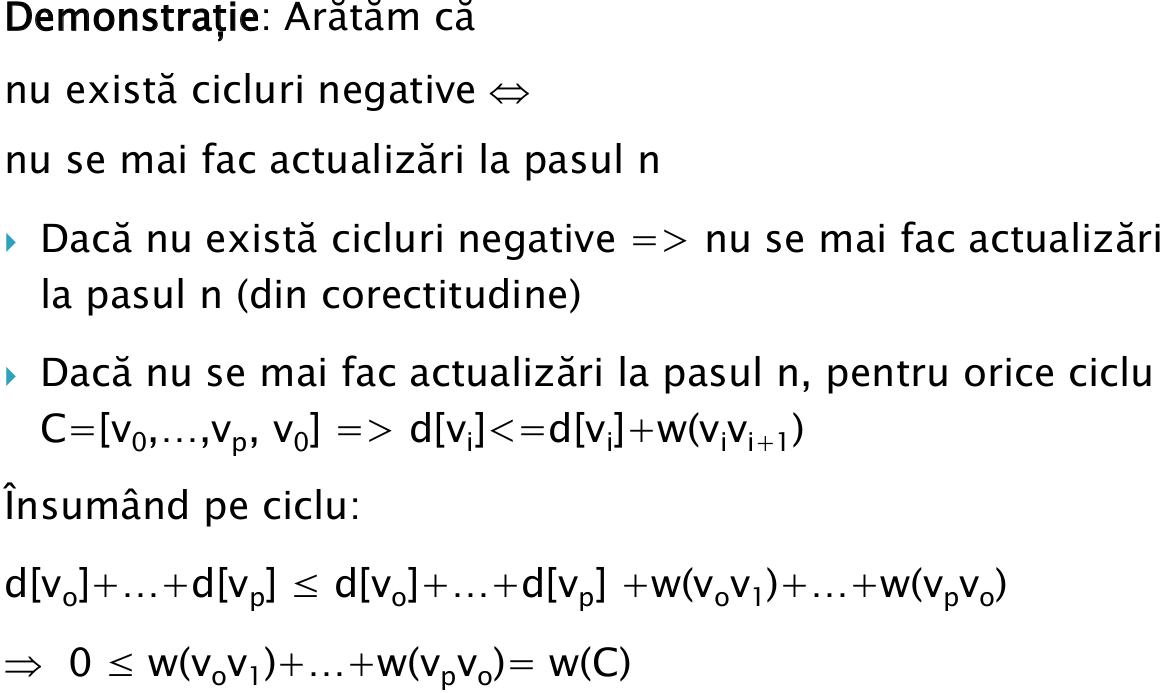
\includegraphics[scale=0.3]{7_bellmanford_circneg.png}
\end{center}

\subparagraph*{Algoritm}Afișarea ciclului negative detectat - folosind tata:
\begin{itemize}
    \item Fie v un vârf al cărei etichetă s-a actualizat la pasul k
    \item  Facem n pași înapoi din v folosind vectorul tata (către s) ; fie x vârful în care am ajuns
    \item Afișăm ciclul care conține pe x folosind tata (din x până ajungem iar în x)
\end{itemize}

\subsection*{Drumuri minime de sursa unica in grafuri aciclice}
\begin{center}
    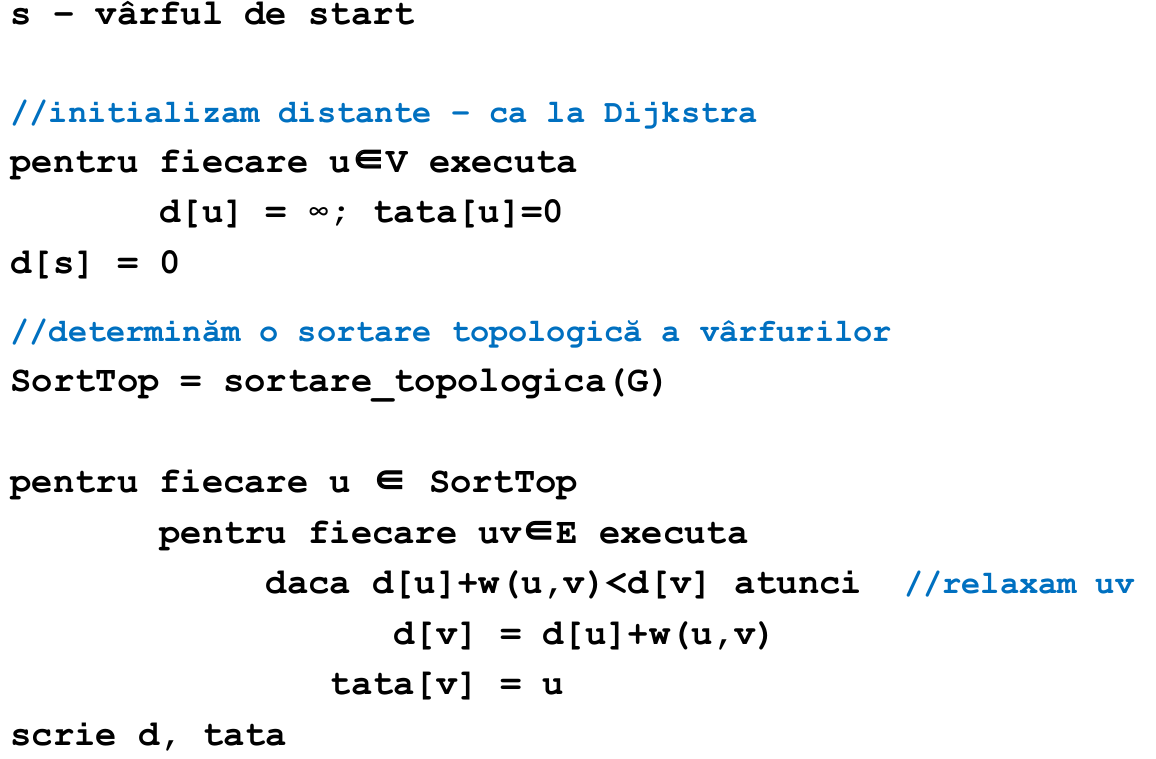
\includegraphics[scale=0.3]{8_drumminim_sursaunica.png}
\end{center}

\paragraph*{Complexitate} $O(V+E)$
\begin{itemize}
    \item Initializare: $O(n)$
    \item Sortare topologica: $O(m+n)$
    \item m * relaxare uv: $O(m)$
\end{itemize}

\section{Drumuri minime intre toate perechile de varfuri}
\subsection*{Floyd-Warshall}
\paragraph*{Complexitate} $O(n^3)$

\begin{lstlisting}
for(i=1;i<=n;i++)
    for(j=1;j<=n;j++){
        d[i][j]=w[i][j]; // adaugam distanta ca fiind greutatea muchiei
        // daca e INF, nu e parinte, altfel il adaugam
        if(w[i][j]== INF)
            p[i][j]=0;
        else
            p[i][j]=i;
    }

    for(k=1;k<=n;k++)
        for(i=1;i<=n;i++)
            for(j=1;j<=n;j++)
                if(d[i][j]>d[i][k]+d[k][j]){ 
                    // Daca ce avem e mai mare decat suma distantelor, actualizam
                    d[i][j]=d[i][k]+d[k][j];
                    p[i][j]=p[k][j];
                }
   \end{lstlisting}

\begin{center}
    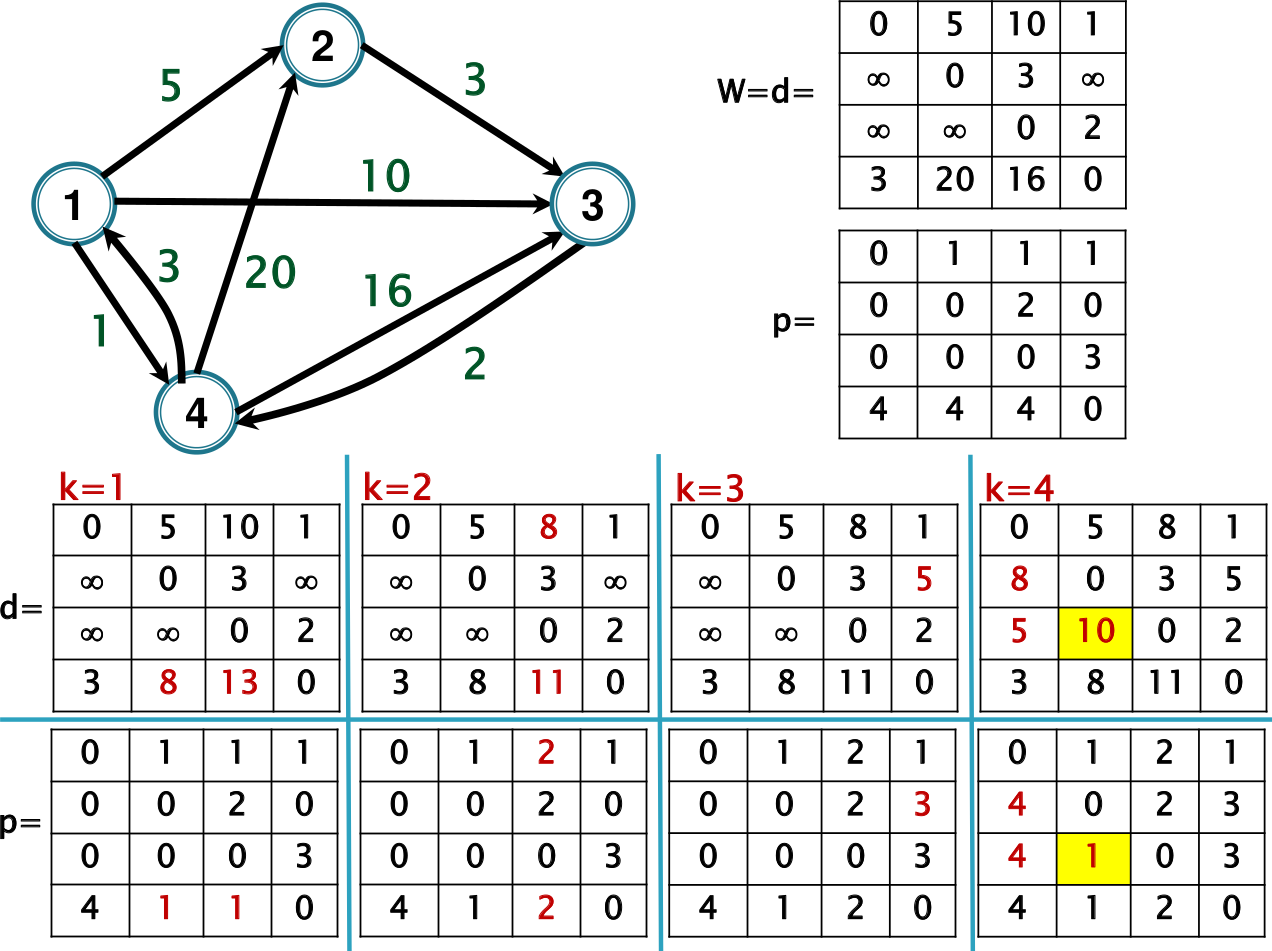
\includegraphics[scale=0.3]{9_floydwarshall.png}
\end{center}

\paragraph*{Inchiderea tranzitiva}
\begin{center}
    \begin{lstlisting}
for(k=1;k<=n;k++)
    for(i=1;i<=n;i++)
        for(j=1;j<=n;j++)
            d[i][j] = d[i][j] || (d[i][k] && d[k][j]);
        \end{lstlisting}
\end{center}

\section{Flow}
\subsection*{Definitii}
\paragraph*{Fie N = (G, {s}, {t}, I, c) o rețea.}
\paragraph*{Lant.} Un s-t lanț este o succesiune de vârfuri distincte și arce din G
\begin{center}
    $P = [ s=v_0, e_1, v_1, …, v_{k-1}, e_k, v_k=t ]$
\end{center}
\paragraph*{Capacitate reziduala a arcului.} Asociem fiecărui arc e din P o pondere, numită capacitate reziduală în P = cu cat mai poate fi modificat fluxul pe arcul e de-a lungul lantului P
\begin{center}
    \[
        i_P(e) = \left\{
        \begin{array}{ll}
            c(e) - f(e), e \ este \ arc \ direct \ in \ P \\
            f(e), e \ este \ arc \ invers \ in \ P
        \end{array}
        \right.
    \]
\end{center}

\paragraph*{Capacitatea reziduala a lantului.} Cu cat poate fi modificat fluxul de-a lungul lantului P.
\begin{center}
    $i(P) = min \{i_P(e) | e \in E(P)\}$
\end{center}
\begin{itemize}
    \item \textbf{f-saturat} daca $i(P)=0$
    \item \textbf{f-nesaturat} daca $i(P) \neq 0$
\end{itemize}

\paragraph*{Flux revizuit de-a lungul lantului P.} Fie P un lant f-nesaturat, definim fluxul revizuit ca $f_P : E \to \mathbb{N}$
\begin{center}
    \[
        f_P(e) = \left\{
        \begin{array}{ll}
            f(e) + i(P), e \ este \ arc \ direct \ in \ P \\
            f(e) - i(P), e \ este \ arc \ invers \ in \ P \\
            f(e), altfel
        \end{array}
        \right.
    \]
\end{center}
\subparagraph*{Proprietate} $val(f_P) = val(f) + i(P) \geq val(f) + 1$

\paragraph*{Taietura in retea.} Fie N = (G, {s}, {t}, I, c) o rețea.\\
O tăietură K = (X, Y) în rețea este o (bi)partiție (X, Y) a mulțimii vârfurilor V, astfel încât $s \in X$ și $t \in Y$.
\subparagraph*{Fie K = (X, Y) o tăietură.} Capacitaeta taieturii = suma arcelor care ies din X catre Y.
\begin{center}
    $c(K) = c(X, Y) = \sum_{x \in X, y \in Y, xy \in E}c(xy)$
\end{center}

\subparagraph*{Informal.} O taietura a grafului reprezinta alegerea unui set de muchii care daca sunt scoase, impart graful in 2 partitii si astfel separa sursa de destinatie. Capacitatea unei taieturi este suma capacitatilor muchiilor care fac parte din taietura

\paragraph*{Taietura minima.} Fie N o retea. O taietura $\widetilde{K}$ se numeste \textbf{taietura minima in N} daca
\begin{center}
    $c(\widetilde{K}) = min \{c(K) | K \ este \ taietura \ in \ N\}$
\end{center}
\subparagraph*{Se poate demonstra: } $val(f) \leq c(\widetilde{K})$

\subsection*{Ford Fulkerson} Complexitate $O(f*E)$
\paragraph*{Exemplu} Fie graful
\begin{center}
    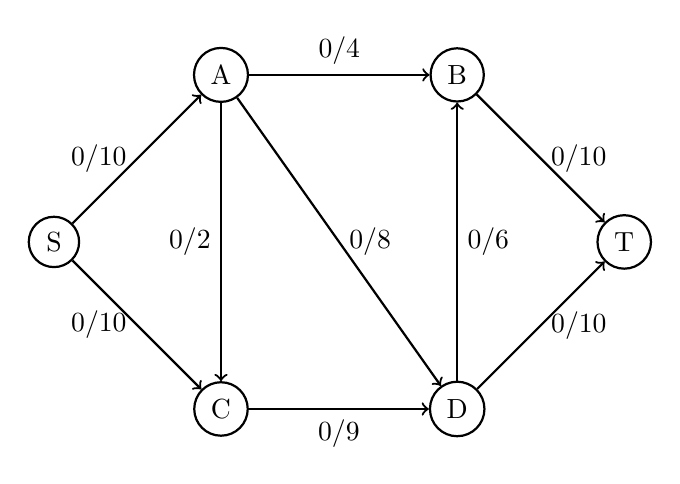
\begin{tikzpicture}[node distance={3cm}, thick, main/.style = {draw, circle}]
        \node[main] (S) {S};
        \node[main] (A) [above right of = S]{A};
        \node[main] (C) [below right of = S]{C};
        \node[main] (B) [right of = A]{B};
        \node[main] (D) [right of = C]{D};
        \node[main] (T) [above right of = D]{T};

        \draw[->] (S) -- (A) node [midway,left] {0/10};
        \draw[->] (S) -- (C) node [midway,left] {0/10};
        \draw[->] (A) -- (C) node [midway,left] {0/2};
        \draw[->] (A) -- (B) node [midway,above] {0/4};
        \draw[->] (C) -- (D) node [midway,below] {0/9};
        \draw[->] (A) -- (D) node [midway,right] {0/8};
        \draw[->] (D) -- (B) node [midway,right] {0/6};
        \draw[->] (B) -- (T) node [midway,right] {0/10};
        \draw[->] (D) -- (T) node [midway,right] {0/10};
    \end{tikzpicture}
\end{center}

\subparagraph*{Fie lantul} S - A - B - T (flow = 4, total = 4)
\begin{center}
    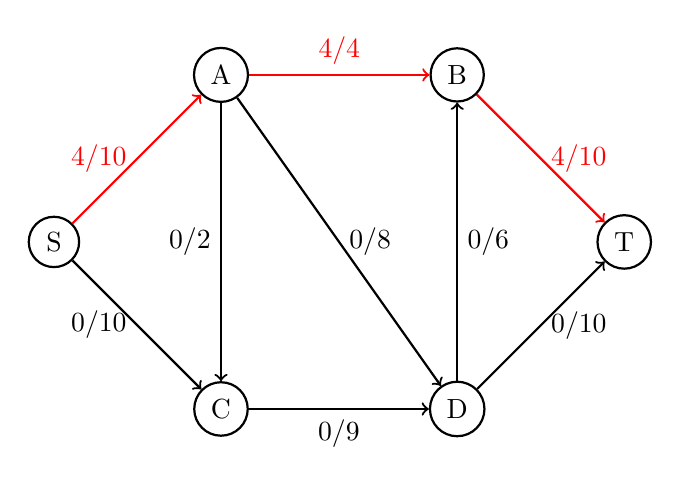
\begin{tikzpicture}[node distance={3cm}, thick, main/.style = {draw, circle}]
        \node[main] (S) {S};
        \node[main] (A) [above right of = S]{A};
        \node[main] (C) [below right of = S]{C};
        \node[main] (B) [right of = A]{B};
        \node[main] (D) [right of = C]{D};
        \node[main] (T) [above right of = D]{T};

        \draw[->, red] (S) -- (A) node [midway,left] {4/10};
        \draw[->] (S) -- (C) node [midway,left] {0/10};
        \draw[->] (A) -- (C) node [midway,left] {0/2};
        \draw[->, red] (A) -- (B) node [midway,above] {4/4};
        \draw[->] (C) -- (D) node [midway,below] {0/9};
        \draw[->] (A) -- (D) node [midway,right] {0/8};
        \draw[->] (D) -- (B) node [midway,right] {0/6};
        \draw[->, red] (B) -- (T) node [midway,right] {4/10};
        \draw[->] (D) -- (T) node [midway,right] {0/10};
    \end{tikzpicture}
\end{center}

\subparagraph*{Fie lantul} S - A - C - D - T (flow = 2, total = 6)
\begin{center}
    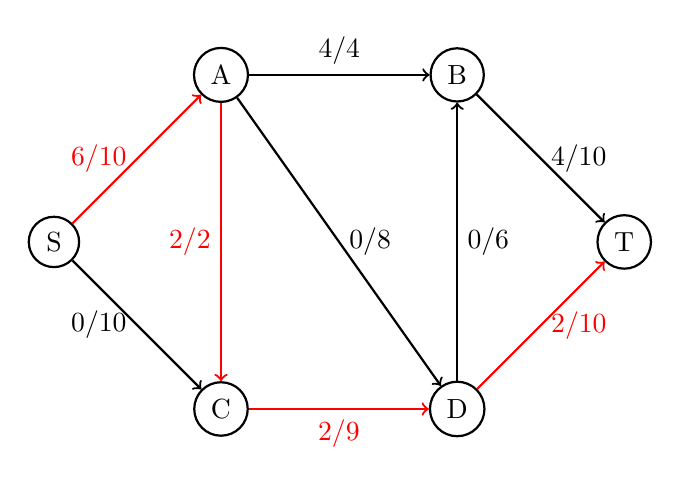
\begin{tikzpicture}[node distance={3cm}, thick, main/.style = {draw, circle}]
        \node[main] (S) {S};
        \node[main] (A) [above right of = S]{A};
        \node[main] (C) [below right of = S]{C};
        \node[main] (B) [right of = A]{B};
        \node[main] (D) [right of = C]{D};
        \node[main] (T) [above right of = D]{T};

        \draw[->, red] (S) -- (A) node [midway,left] {6/10};
        \draw[->] (S) -- (C) node [midway,left] {0/10};
        \draw[->, red] (A) -- (C) node [midway,left] {2/2};
        \draw[->] (A) -- (B) node [midway,above] {4/4};
        \draw[->, red] (C) -- (D) node [midway,below] {2/9};
        \draw[->] (A) -- (D) node [midway,right] {0/8};
        \draw[->] (D) -- (B) node [midway,right] {0/6};
        \draw[->] (B) -- (T) node [midway,right] {4/10};
        \draw[->, red] (D) -- (T) node [midway,right] {2/10};
    \end{tikzpicture}
\end{center}

\subparagraph*{Fie lantul} S - C - D - T (flow = 7, total = 13)
\begin{center}
    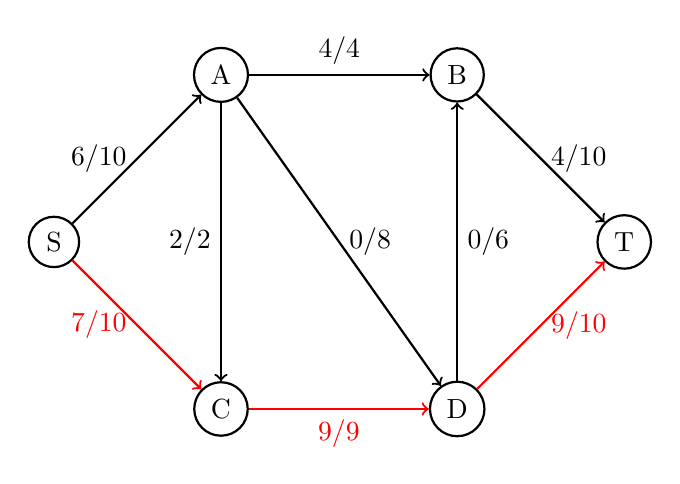
\begin{tikzpicture}[node distance={3cm}, thick, main/.style = {draw, circle}]
        \node[main] (S) {S};
        \node[main] (A) [above right of = S]{A};
        \node[main] (C) [below right of = S]{C};
        \node[main] (B) [right of = A]{B};
        \node[main] (D) [right of = C]{D};
        \node[main] (T) [above right of = D]{T};

        \draw[->] (S) -- (A) node [midway,left] {6/10};
        \draw[->, red] (S) -- (C) node [midway,left] {7/10};
        \draw[->] (A) -- (C) node [midway,left] {2/2};
        \draw[->] (A) -- (B) node [midway,above] {4/4};
        \draw[->, red] (C) -- (D) node [midway,below] {9/9};
        \draw[->] (A) -- (D) node [midway,right] {0/8};
        \draw[->] (D) -- (B) node [midway,right] {0/6};
        \draw[->] (B) -- (T) node [midway,right] {4/10};
        \draw[->, red] (D) -- (T) node [midway,right] {9/10};
    \end{tikzpicture}
\end{center}

\subparagraph*{Fie lantul} S - C - A - D - T (flow = 1, total = 14)
\begin{center}
    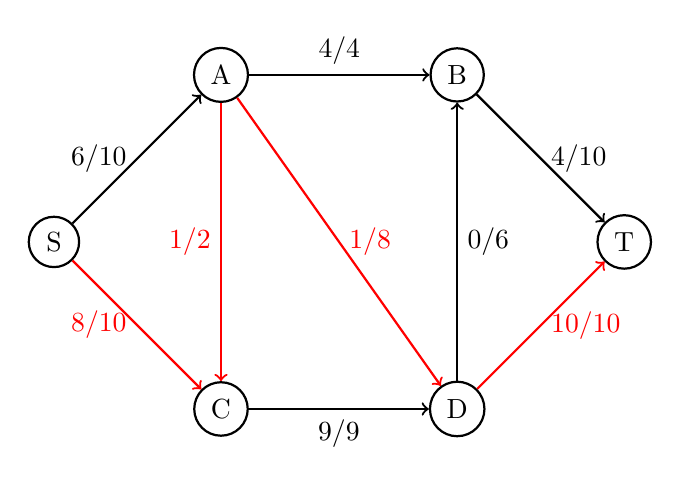
\begin{tikzpicture}[node distance={3cm}, thick, main/.style = {draw, circle}]
        \node[main] (S) {S};
        \node[main] (A) [above right of = S]{A};
        \node[main] (C) [below right of = S]{C};
        \node[main] (B) [right of = A]{B};
        \node[main] (D) [right of = C]{D};
        \node[main] (T) [above right of = D]{T};

        \draw[->] (S) -- (A) node [midway,left] {6/10};
        \draw[->, red] (S) -- (C) node [midway,left] {8/10};
        \draw[->, red] (A) -- (C) node [midway,left] {1/2};
        \draw[->] (A) -- (B) node [midway,above] {4/4};
        \draw[->] (C) -- (D) node [midway,below] {9/9};
        \draw[->, red] (A) -- (D) node [midway,right] {1/8};
        \draw[->] (D) -- (B) node [midway,right] {0/6};
        \draw[->] (B) -- (T) node [midway,right] {4/10};
        \draw[->, red] (D) -- (T) node [midway,right] {10/10};
    \end{tikzpicture}
\end{center}

\subparagraph*{Fie lantul} S - A - D - B - T (flow = 4, total = 18)
\begin{center}
    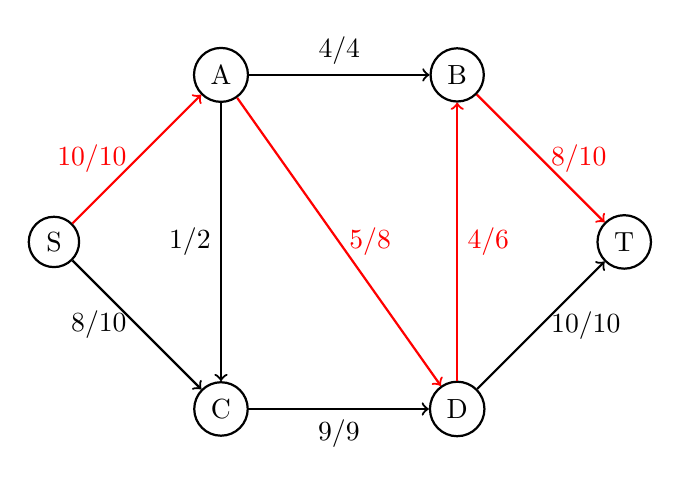
\begin{tikzpicture}[node distance={3cm}, thick, main/.style = {draw, circle}]
        \node[main] (S) {S};
        \node[main] (A) [above right of = S]{A};
        \node[main] (C) [below right of = S]{C};
        \node[main] (B) [right of = A]{B};
        \node[main] (D) [right of = C]{D};
        \node[main] (T) [above right of = D]{T};

        \draw[->, red] (S) -- (A) node [midway,left] {10/10};
        \draw[->] (S) -- (C) node [midway,left] {8/10};
        \draw[->] (A) -- (C) node [midway,left] {1/2};
        \draw[->] (A) -- (B) node [midway,above] {4/4};
        \draw[->] (C) -- (D) node [midway,below] {9/9};
        \draw[->, red] (A) -- (D) node [midway,right] {5/8};
        \draw[->, red] (D) -- (B) node [midway,right] {4/6};
        \draw[->, red] (B) -- (T) node [midway,right] {8/10};
        \draw[->] (D) -- (T) node [midway,right] {10/10};
    \end{tikzpicture}
\end{center}

\subparagraph*{Fie lantul} S - C - A - D - B - T (flow = 1, total = 19)
\begin{center}
    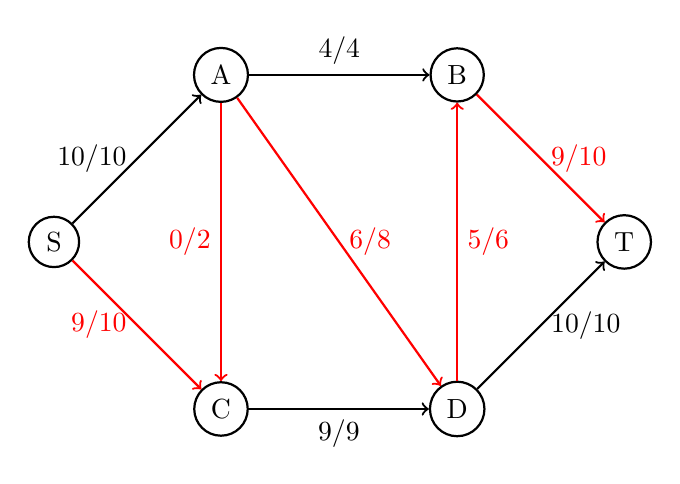
\begin{tikzpicture}[node distance={3cm}, thick, main/.style = {draw, circle}]
        \node[main] (S) {S};
        \node[main] (A) [above right of = S]{A};
        \node[main] (C) [below right of = S]{C};
        \node[main] (B) [right of = A]{B};
        \node[main] (D) [right of = C]{D};
        \node[main] (T) [above right of = D]{T};

        \draw[->] (S) -- (A) node [midway,left] {10/10};
        \draw[->, red] (S) -- (C) node [midway,left] {9/10};
        \draw[->, red] (A) -- (C) node [midway,left] {0/2};
        \draw[->] (A) -- (B) node [midway,above] {4/4};
        \draw[->] (C) -- (D) node [midway,below] {9/9};
        \draw[->, red] (A) -- (D) node [midway,right] {6/8};
        \draw[->, red] (D) -- (B) node [midway,right] {5/6};
        \draw[->, red] (B) -- (T) node [midway,right] {9/10};
        \draw[->] (D) -- (T) node [midway,right] {10/10};
    \end{tikzpicture}
\end{center}

\subparagraph*{Nu mai avem drumuri de la S la T, deci flow total = 19}

\subsection*{Edmonds-Karp} Complexitate $O(V*E^2)$
\paragraph*{Exemplu} Fie graful
\begin{center}
    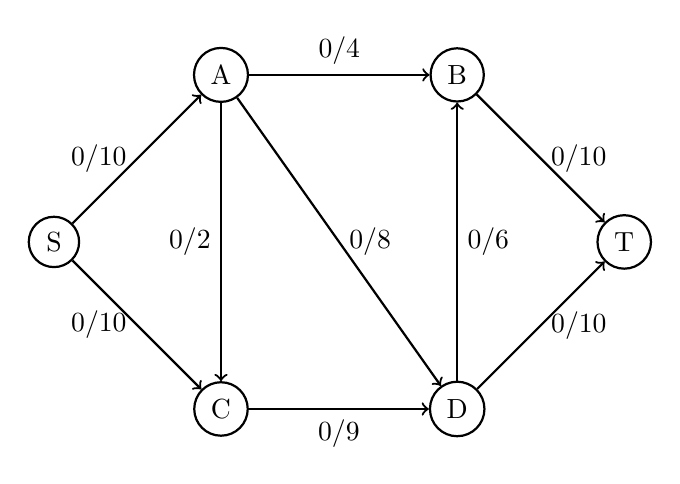
\begin{tikzpicture}[node distance={3cm}, thick, main/.style = {draw, circle}]
        \node[main] (S) {S};
        \node[main] (A) [above right of = S]{A};
        \node[main] (C) [below right of = S]{C};
        \node[main] (B) [right of = A]{B};
        \node[main] (D) [right of = C]{D};
        \node[main] (T) [above right of = D]{T};

        \draw[->] (S) -- (A) node [midway,left] {0/10};
        \draw[->] (S) -- (C) node [midway,left] {0/10};
        \draw[->] (A) -- (C) node [midway,left] {0/2};
        \draw[->] (A) -- (B) node [midway,above] {0/4};
        \draw[->] (C) -- (D) node [midway,below] {0/9};
        \draw[->] (A) -- (D) node [midway,right] {0/8};
        \draw[->] (D) -- (B) node [midway,right] {0/6};
        \draw[->] (B) -- (T) node [midway,right] {0/10};
        \draw[->] (D) -- (T) node [midway,right] {0/10};
    \end{tikzpicture}
\end{center}

\subparagraph*{Parcurgerea BFS} Flow = 4, Total = 4
\begin{center}
    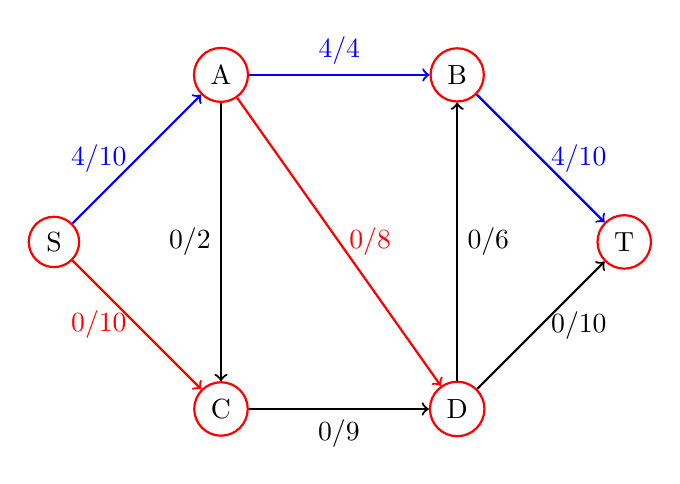
\begin{tikzpicture}[node distance={3cm}, thick, main/.style = {draw, circle}]
        \node[red state] (S) {S};
        \node[red state] (A) [above right of = S]{A};
        \node[red state] (C) [below right of = S]{C};
        \node[red state] (B) [right of = A]{B};
        \node[red state] (D) [right of = C]{D};
        \node[red state] (T) [above right of = D]{T};

        \draw[->, blue] (S) -- (A) node [midway,left] {4/10};
        \draw[->, red] (S) -- (C) node [midway,left] {0/10};
        \draw[->] (A) -- (C) node [midway,left] {0/2};
        \draw[->, blue] (A) -- (B) node [midway,above] {4/4};
        \draw[->] (C) -- (D) node [midway,below] {0/9};
        \draw[->, red] (A) -- (D) node [midway,right] {0/8};
        \draw[->] (D) -- (B) node [midway,right] {0/6};
        \draw[->, blue] (B) -- (T) node [midway,right] {4/10};
        \draw[->] (D) -- (T) node [midway,right] {0/10};
    \end{tikzpicture}
\end{center}

\subparagraph*{Parcurgerea BFS} Flow = 6, Total = 10
\begin{center}
    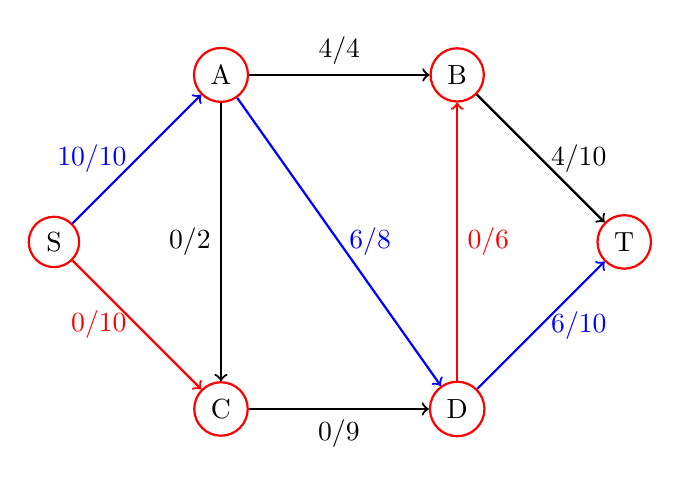
\begin{tikzpicture}[node distance={3cm}, thick, main/.style = {draw, circle}]
        \node[red state] (S) {S};
        \node[red state] (A) [above right of = S]{A};
        \node[red state] (C) [below right of = S]{C};
        \node[red state] (B) [right of = A]{B};
        \node[red state] (D) [right of = C]{D};
        \node[red state] (T) [above right of = D]{T};

        \draw[->, blue] (S) -- (A) node [midway,left] {10/10};
        \draw[->, red] (S) -- (C) node [midway,left] {0/10};
        \draw[->] (A) -- (C) node [midway,left] {0/2};
        \draw[->] (A) -- (B) node [midway,above] {4/4};
        \draw[->] (C) -- (D) node [midway,below] {0/9};
        \draw[->, blue] (A) -- (D) node [midway,right] {6/8};
        \draw[->, red] (D) -- (B) node [midway,right] {0/6};
        \draw[->] (B) -- (T) node [midway,right] {4/10};
        \draw[->, blue] (D) -- (T) node [midway,right] {6/10};
    \end{tikzpicture}
\end{center}

\subparagraph*{Parcurgerea BFS} Flow = 4, Total = 14
\begin{center}
    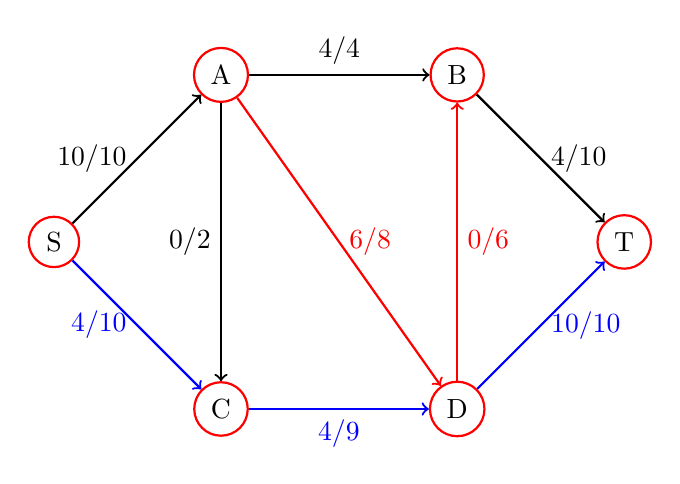
\begin{tikzpicture}[node distance={3cm}, thick, main/.style = {draw, circle}]
        \node[red state] (S) {S};
        \node[red state] (A) [above right of = S]{A};
        \node[red state] (C) [below right of = S]{C};
        \node[red state] (B) [right of = A]{B};
        \node[red state] (D) [right of = C]{D};
        \node[red state] (T) [above right of = D]{T};

        \draw[->] (S) -- (A) node [midway,left] {10/10};
        \draw[->, blue] (S) -- (C) node [midway,left] {4/10};
        \draw[->] (A) -- (C) node [midway,left] {0/2};
        \draw[->] (A) -- (B) node [midway,above] {4/4};
        \draw[->, blue] (C) -- (D) node [midway,below] {4/9};
        \draw[->, red] (A) -- (D) node [midway,right] {6/8};
        \draw[->, red] (D) -- (B) node [midway,right] {0/6};
        \draw[->] (B) -- (T) node [midway,right] {4/10};
        \draw[->, blue] (D) -- (T) node [midway,right] {10/10};
    \end{tikzpicture}
\end{center}

\subparagraph*{Parcurgerea BFS} Flow = 5, Total = 19
\begin{center}
    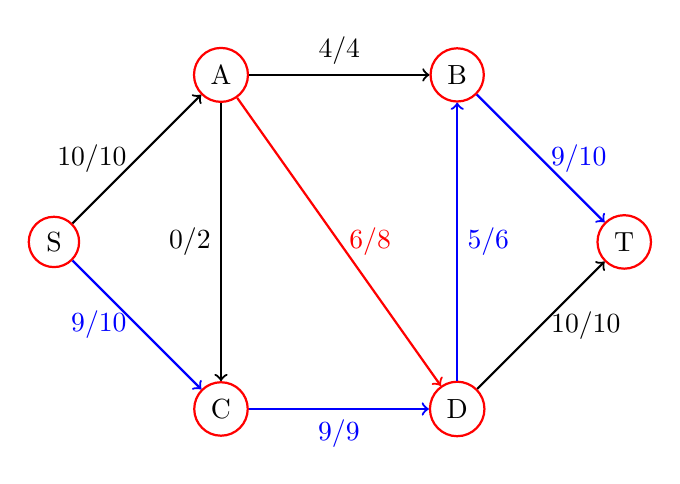
\begin{tikzpicture}[node distance={3cm}, thick, main/.style = {draw, circle}]
        \node[red state] (S) {S};
        \node[red state] (A) [above right of = S]{A};
        \node[red state] (C) [below right of = S]{C};
        \node[red state] (B) [right of = A]{B};
        \node[red state] (D) [right of = C]{D};
        \node[red state] (T) [above right of = D]{T};

        \draw[->] (S) -- (A) node [midway,left] {10/10};
        \draw[->, blue] (S) -- (C) node [midway,left] {9/10};
        \draw[->] (A) -- (C) node [midway,left] {0/2};
        \draw[->] (A) -- (B) node [midway,above] {4/4};
        \draw[->, blue] (C) -- (D) node [midway,below] {9/9};
        \draw[->, red] (A) -- (D) node [midway,right] {6/8};
        \draw[->, blue] (D) -- (B) node [midway,right] {5/6};
        \draw[->, blue] (B) -- (T) node [midway,right] {9/10};
        \draw[->] (D) -- (T) node [midway,right] {10/10};
    \end{tikzpicture}
\end{center}

\begin{center}
    \textbf{Nu mai putem parcurge BFS, asa ca avem flow total 19}
\end{center}

\section{Grafuri bipartite}
\paragraph*{Definitie.}G = (V, E) graf neorientat s.n. bipartit $\Leftrightarrow$ există o partiție a lui V în două submulțimi V1, V2 (bipartiție):
\begin{center}
    $V = V_1 \cup V_2$\\
    $V_1 \cap V_2 = \varnothing$
\end{center}
astfel încât orice muchie $e \in E$ are o extremitate în $V_1$ și cealaltă în $V_2$
\begin{center}
    Notăm $G = (V1 \cup V2, E)$
\end{center}
\paragraph*{Bipartit complet.} $G=(V,E)$ este bipartit complet $\Leftrightarrow$ este bipartit si $E=\{xy | x \in V_1, y \in V_2 \}$
\begin{center}
    Notam cu $K_{p,q}$ daca $p = |V_1|$ si $q = |V_2|$
\end{center}
\subparagraph*{Numarul maxim de muchii:} $\lfloor\frac{N^2}{4}\rfloor$

\paragraph*{Observatie.} G = (V, E) bipartit $\Leftrightarrow$ există o 2-colorare proprie a vârfurilor (bicolorare): $c:V \rightarrow \{1,2\}$ (adica pentru orice muchie $e = xy \in E$, avem $c(x) \neq c(y)$)

\paragraph*{Teorema König.} Fie $G = (V, E)$ un graf cu $n \geq 2$ vârfuri. Avem G este bipartit $\Leftrightarrow$ toate ciclurile elementare din G sunt pare.
\subparagraph*{Algoritm pentru testare.}
\begin{itemize}
    \item Colorăm cu 2 culori un arbore parțial al său printr-o parcurgere (colorăm orice vecin j nevizitat al vârfului curent i cu o culoare
          diferită de cea a lui i)
    \item Testăm dacă celelalte muchii – de la i la vecini j deja vizitați (colorați) au extremitățile i și j colorate diferit
\end{itemize}


\subsection*{Cuplaj maxim in grafuri bipartite}
\paragraph*{Definitii.} Fie $G = (V, E)$ un graf şi $M \subseteq E$.
\begin{itemize}
    \item M s.n cuplaj dacă orice două muchii din M sunt neadiacente
    \item V(M) = mulţimea vârfurilor M-saturate
    \item V(G) - V(M) = mulţimea vârfurilor M-nesaturate
\end{itemize}

\subparagraph*{} Un cuplaj $M^*$ s.n cuplaj de cardinal maxim (cuplaj maxim):
\begin{center}
    $| M^*| \geq |M|,  \forall M \subseteq E\ cuplaj$
\end{center}

\paragraph*{Algoritm de determinare.}
\begin{itemize}
    \item Reducem problema determinării unui cuplaj maxim într-un cuplaj bipartit G la determinarea unui flux maxim într-o rețea de transport asociată lui G
    \item Construim rețeaua de transport $N_G$ asociată lui G
    \item Adăugăm două noduri noi s şi t
    \item Adăugăm arce $(s,x_i)$, pentru $x_i \in X$ şi $(y_j, t)$, $y_j \in Y$
    \item Transformăm muchiile $x_iy_j$ în arce (de la X la Y)
    \item Asociem fiecărui arc capacitatea 1
    \item Cuplaj M în G $\Leftrightarrow$ flux f în rețea
    \item $|M|=val(f)$
\end{itemize}

\paragraph*{Proprietati}
\subparagraph*{Proprietatea 1.} Fie $G=(X \cup Y, E)$ un graf bipartit şi M un cuplaj în G. Atunci există un flux f în reţeaua de transport asociată $N_G$ cu
\begin{center}
    $val(f) = |M|$
\end{center}

\subparagraph*{Proprietatea 2.} Fie $G=(X \cup Y, E)$ un graf bipartit şi f un flux în reţeaua de transport $N_G$ asociată. Atunci există M un cuplaj în G cu
\begin{center}
    $val(f) = |M|$
\end{center}

\paragraph*{Consecinta.} $f^*$ flux maxim în N $\Rightarrow$ cuplajul corespunzător $M^*$ este cuplaj maxim în G \\
A determina un cuplaj maxim într-un graf bipartit $\Leftrightarrow$ a determina un flux maxim în reţeaua asociată

\paragraph*{Algoritm.} Complexitate: C=1 (sau $L \leq c^+(s) \leq n$) $\Rightarrow$ O(mn). Fie $G = (X \cup Y, E)$
\begin{itemize}
    \item Construim N reţeaua de transport asociată
    \item Determinăm $f^*$ flux maxim în N
    \item Considerăm $M = \{xy| f^*(xy)=1, x \in X, y \in Y, xy \in N \}$ (pentru fiecare arc cu flux nenul xy din N care nu este incident în s sau t, muchia xy corespunzătoare din G se adaugă la M)
    \item return M
\end{itemize}

\section{Grafuri Euleriene}
\paragraph*{Ciclu eulerian:} traseu închis care trece o singură dată prin toate muchiile
\paragraph*{Graf eulerian:} conține un ciclu eulerian
\paragraph*{Lant eulerian:} Lanț eulerian al lui G = lanț simplu P în G cu $E(P) = E(G)$

\paragraph*{Lema} Fie $G=(V,E)$ un graf neorientat, conex, cu toate vârfurile de
grad par și $E \neq \varnothing$. Atunci pentru orice $x \in V$ există un ciclu C în G cu $x \in V(C)$ (ciclu care conține x, nu neapărat eulerian, nici neapărat elementar).

\begin{center}
    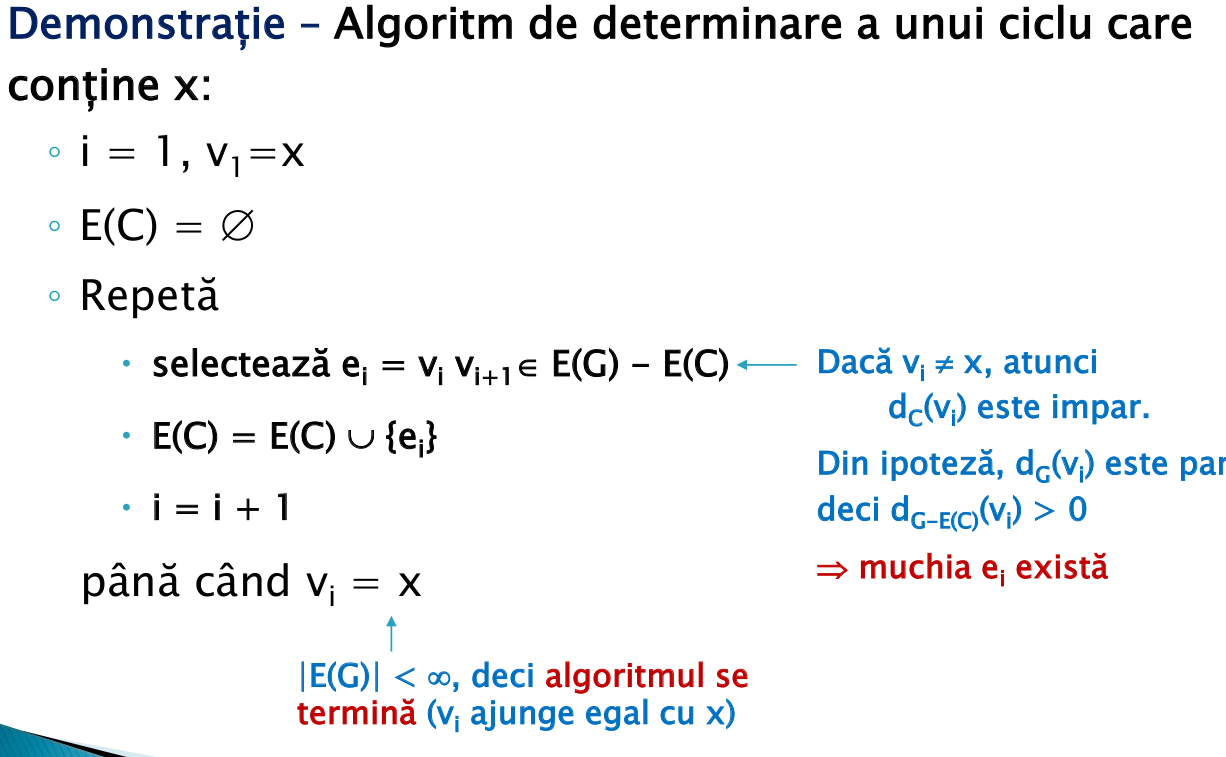
\includegraphics[scale=0.3]{10_grafeulerian.png}
\end{center}

\begin{center}
    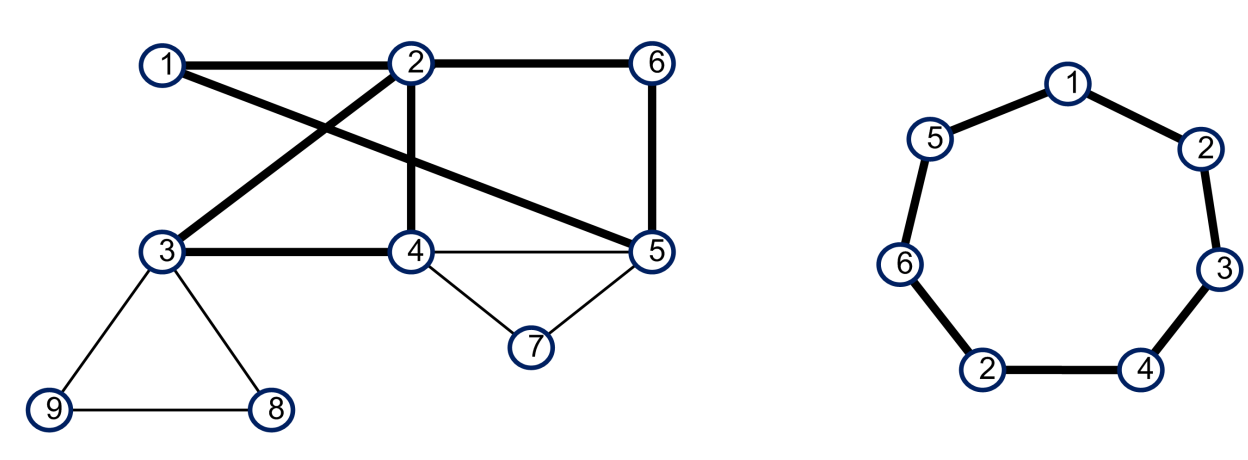
\includegraphics[scale=0.3]{11_determinare_ciclueulerian.png}
\end{center}

\paragraph*{Teorema lui Euler.} Fie $G=(V, E)$ un (multi)graf neorientat, conex, cu $E \neq \varnothing$. Atunci G este eulerian $\Leftrightarrow$ orice varf din G are grad par.

\paragraph*{Hierholzer.} Complexitate $O(m)$. Determinarea unui ciclu eulerian într-un graf conex (sau un
graf conex+ vârfuri izolate) cu toate vârfurile de grad par
\begin{center}
    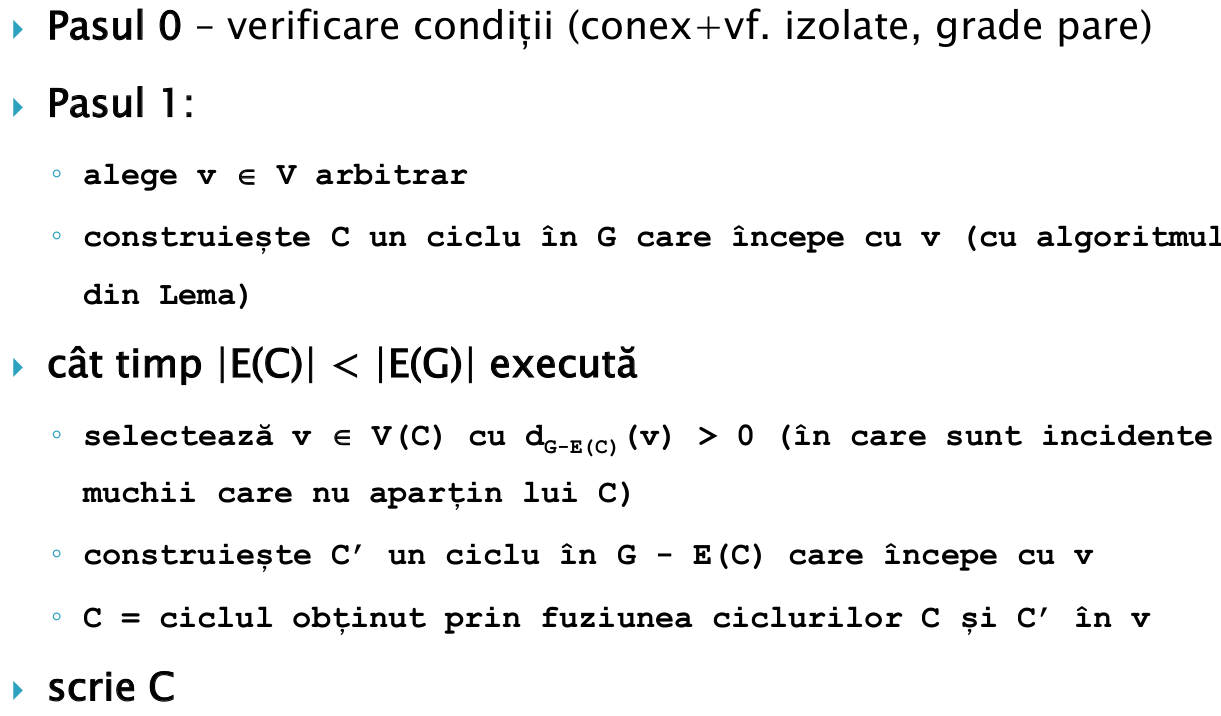
\includegraphics[scale=0.3]{12_hierholzer.png}
\end{center}
\begin{center}
    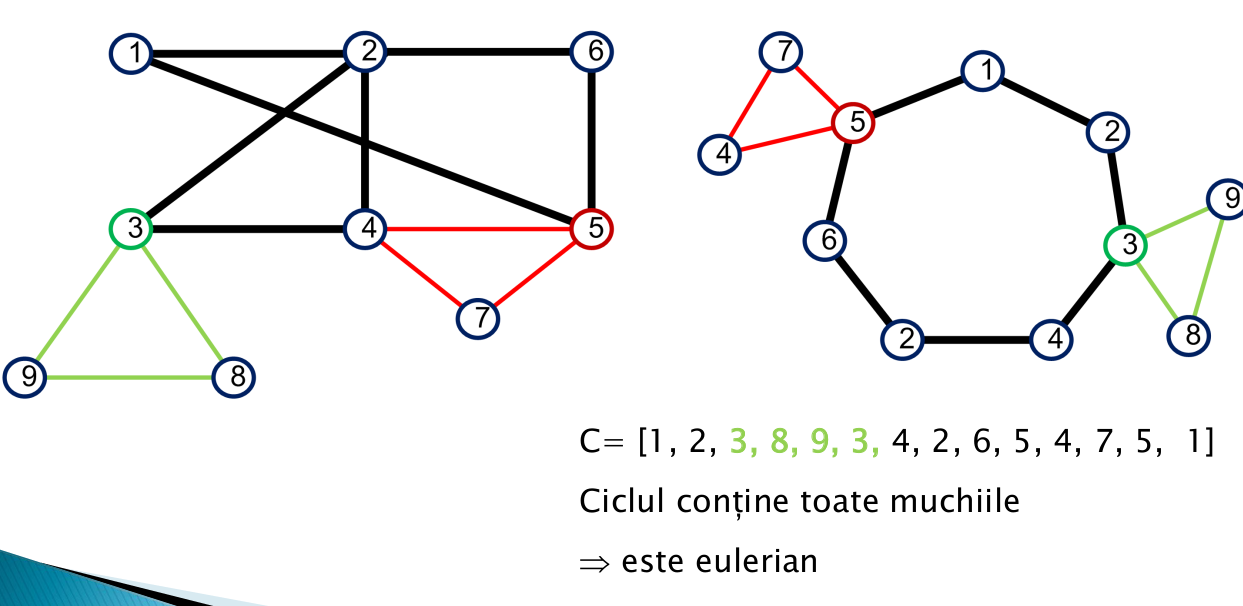
\includegraphics[scale=0.3]{13_hierholzer_graf.png}
\end{center}

\section{Grafuri planare}
\paragraph*{Definitie.} $G = (V, E)$ graf neorientat s.n. planar $\Leftrightarrow$ admite o reprezentare în plan a.î. muchiilor le corespund segmente de curbe continue care nu se intersectează în interior unele pe altele
\paragraph*{Harta.} Fie $G = (V, E)$ graf planar, M o hartă a sa. M induce o împărțire a planului într-o mulțime F de părți convexe numite fețe. Una dintre acestea este fața infinită (exterioară).
\begin{itemize}
    \item $M = (V, E, F)$ hartă
    \item Pentru o față $f \in F$ definim: $d_M(f)$ = gradul feței f = numărul muchiilor lanțului închis (frontierei) care delimitează f (câte muchii sunt parcurse atunci când traversăm frontiera)
    \item $\sum_{f \in F} d_M(f) = 2 * |E|$
\end{itemize}

\paragraph*{Teorema poliedrală a lui Euler.} Fie $G=(V, E)$ un graf planar conex și $M = (V, E, F)$ o harta a lui. Are loc relația $|V| - |E| + |F| = 2$
\subparagraph*{Consecinta:} Orice hartă M a lui G are $2 - |V| + |E|$ fețe
\paragraph*{Teorema celor 6 culori.} Orice graf planar conex este 6 – colorabil.
\begin{center}
    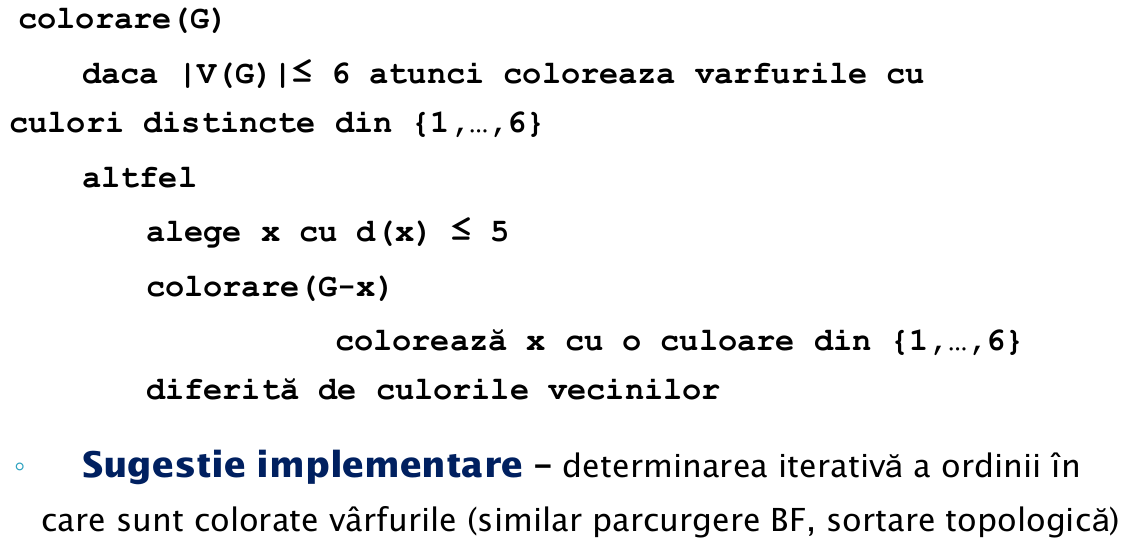
\includegraphics[scale=0.3]{14_grafplanar_6colorabil.png}
\end{center}

\paragraph*{Teorema lui Kuratowski.} Un graf este non-planar $\Leftrightarrow$ contine un subgraf homomorf cu $K_5$ sau $K_{3,3}$

\paragraph*{Loop free planar graph.} Fie un graf planar cu $|V|=v$ si $|E|=e \ge 2$, atunci  $3*r \leq 2*e$ si $e \leq 3*v-6$

\section{Grafuri Hamiltoniene}
\paragraph*{Definitie.} Un graf este hamiltonian dacă admite un ciclu hamiltonian adică un ciclu care contine toate nodurile grafului.
\paragraph*{Conditie necesara.} Grafurile hamiltoniene sunt biconexe(nu are noduri critice). Inversa nu este adevarata.
\paragraph*{Teorema lui Dirac.} Fie G un graf cu ordinul $n \geq 3$. Dacă $\delta (G) \geq n/2$ atunci G este hamiltonian.

\paragraph*{Teorema lui Ore.} Fie G un graf cu ordinul $n \geq 3$, dacă avem pentru oricare pereche de noduri neadiacente $deg(x) + deg(y) \geq n$ $\rightarrow$ atunci graful este Hamiltonian.

\paragraph*{Definitii ajutatoare.} Conectivitatea $K(G)$ unui graf G este este marimea minima a unei mulțimi de tăiere a lui G.\\
Se calculeaza prin: Flux maxim = taietura minima
\subparagraph*{} O mulțime de noduri a unui graf G este independentă dacă nu contine
noduri adiacente. Numărul de independență $\alpha (G)$ al unui graf G este marimea cea mai mare posibila a unei mulțimi independente a lui G

\paragraph*{Teorema lui Chvatal si Erdos.} Fie G un graf conectat cu ordinul $n \geq 3$, conectivitatea $K(G)$, și numărul de independență $\alpha(G)$. Daca $K(G) \geq \alpha(G)$, atunci G este hamiltonian.

\paragraph*{Teorema lui Goodman si Hedetniemi.} Daca G este un graf 2-conectat si liber de $\{K_{1,3}, Z_1\}$ atunci G este hamiltonian

\end{document}